\documentclass[journal]{IEEEtran}
\usepackage[T1]{fontenc}
\usepackage[utf8]{inputenc}
\usepackage{amsmath,amssymb,amsfonts}
\usepackage{graphicx,booktabs,array,tabularx,multirow}
\usepackage{xurl}
\usepackage{xcolor,url,cite,microtype}
\usepackage[caption=false,font=footnotesize]{subfig}
\usepackage[hidelinks]{hyperref}
\hypersetup{pdftitle={A Comprehensive Survey of Diffusion-based Video Restoration and Enhancement},pdfauthor={Han Zhang; Yiang Chen; Zengyuan Zuo; Kui Jiang; Junjun Jiang; Xianming Liu},pdfsubject={Diffusion-based video restoration and enhancement},pdfkeywords={video restoration, diffusion, temporal consistency, video quality assessment}}
\newcolumntype{Y}{>{\raggedright\arraybackslash}X}
\newcommand{\R}{\mathbb{R}}
\newcommand{\E}{\mathbb{E}}
\setlength{\emergencystretch}{1em}
\hyphenation{dif-fu-sion re-sto-ra-tion spatio-temporal}
\begin{document}
\bstctlcite{bstcontrol}
\title{A Comprehensive Survey of Diffusion-based Video\\Restoration and Enhancement}
\author{Han~Zhang, Yiang~Chen, Zengyuan~Zuo, Kui~Jiang, Junjun~Jiang,~\IEEEmembership{Senior Member,~IEEE}, and Xianming~Liu,~\IEEEmembership{Member,~IEEE}
\thanks{H. Zhang, Y. Chen, Z. Zuo, K. Jiang, J. Jiang, and X. Liu are with the School of Computer Science and Technology, Harbin Institute of Technology, Harbin 150001, China. Corresponding author: Kui Jiang (jiangkui@hit.edu.cn).}}
\markboth{Journal of \LaTeX\ Class Files,~Vol.~14, No.~8, August~2021}%
{Shell \MakeLowercase{\textit{et al.}}: A Comprehensive Survey of Diffusion-based Video Restoration and Enhancement}
\maketitle
\begin{abstract}
Video restoration and enhancement recover visual information from sequences affected by limited resolution, noise, blur, compression, and challenging imaging conditions. Diffusion models offer expressive generative priors for reconstructing realistic detail, while introducing new challenges in preserving fidelity and temporal consistency. This survey presents a comprehensive overview of diffusion-based video restoration and enhancement, organized around the interaction of perceptual quality, fidelity, and temporal coherence. We establish a unified taxonomy of degradation assumptions, learning strategies, generative priors, conditioning mechanisms, temporal modeling, inference efficiency, and system paradigms. We review pretrained image and video priors, restoration-trained diffusion models, and related flow-matching formulations, with a focus on how these methods preserve temporal consistency. The discussion covers super-resolution, generic restoration, deblurring, adverse-weather removal, low-light and underwater enhancement, compression artifact reduction, face restoration, inpainting, and generated-video enhancement. We further examine datasets and evaluation metrics, with particular attention to backbone differences, metric reliability, and the distinction between method-level and system-level comparisons. Finally, we discuss challenges and future directions in controllable restoration, long-video processing, physically grounded enhancement, efficient deployment, and generalist restoration systems.
\end{abstract}
\begin{IEEEkeywords}
Video restoration, diffusion models, generative priors, temporal consistency, video quality assessment.
\end{IEEEkeywords}
\section{Introduction}
\label{sec:intro}
\IEEEPARstart{V}{ideo} restoration and enhancement aim to improve visual information acquired under imperfect imaging, transmission, and generation conditions. Limited spatial resolution, sensor noise, motion blur, compression, and adverse illumination can obscure both the appearance of a scene and its evolution over time. The problem extends beyond natural RGB video to faces, underwater scenes, infrared imaging, high-dynamic-range content, and AI-generated video. Across these settings, a useful reconstruction must recover detail while preserving the structures and events represented by the input.

Temporal redundancy distinguishes video restoration from its image counterpart. Neighboring frames can reveal complementary texture, compensate for occlusion, and constrain motion, enabling alignment, propagation, recurrence, and attention to improve reconstruction~\cite{vrsurvey,realbasicvsr}. However, information lost across an entire sequence remains difficult to recover. Under severe degradation, minimizing pixel-wise error often favors averaged, oversmoothed predictions. Perceptual and adversarial objectives address this limitation by encouraging realistic appearance. Diffusion models offer a further route through expressive, reusable image and video priors~\cite{ddpm,ldm,svd,wan}. Their success has motivated methods for real-world video super-resolution (VSR), generic restoration, and specialized enhancement~\cite{upscale,stablevsr,seedvr,undive}.

The use of generative priors changes the central restoration problem. A detailed frame can contain plausible texture that differs from the underlying scene, and independently synthesized textures can vary across frames even when the scene does not. Conversely, a temporally smooth reconstruction may preserve an incorrect face or suppress genuine motion. Diffusion-based video restoration consequently involves three closely related objectives: \emph{fidelity} to the observed scene, \emph{perceptual quality} of the reconstructed content, and \emph{temporal consistency} of appearance, geometry, identity, and motion. The published examples in Fig.~\ref{fig:tradeoff} make these distinctions visible. These objectives are not always aligned. Improving perceptual quality may increase reconstruction error, as described by the perception–distortion tradeoff. In video, generated details may also vary across frames, introducing flicker and temporal inconsistency. The central challenge is therefore to balance perceptual quality, fidelity, and temporal consistency.

\begin{figure*}[t]
\centering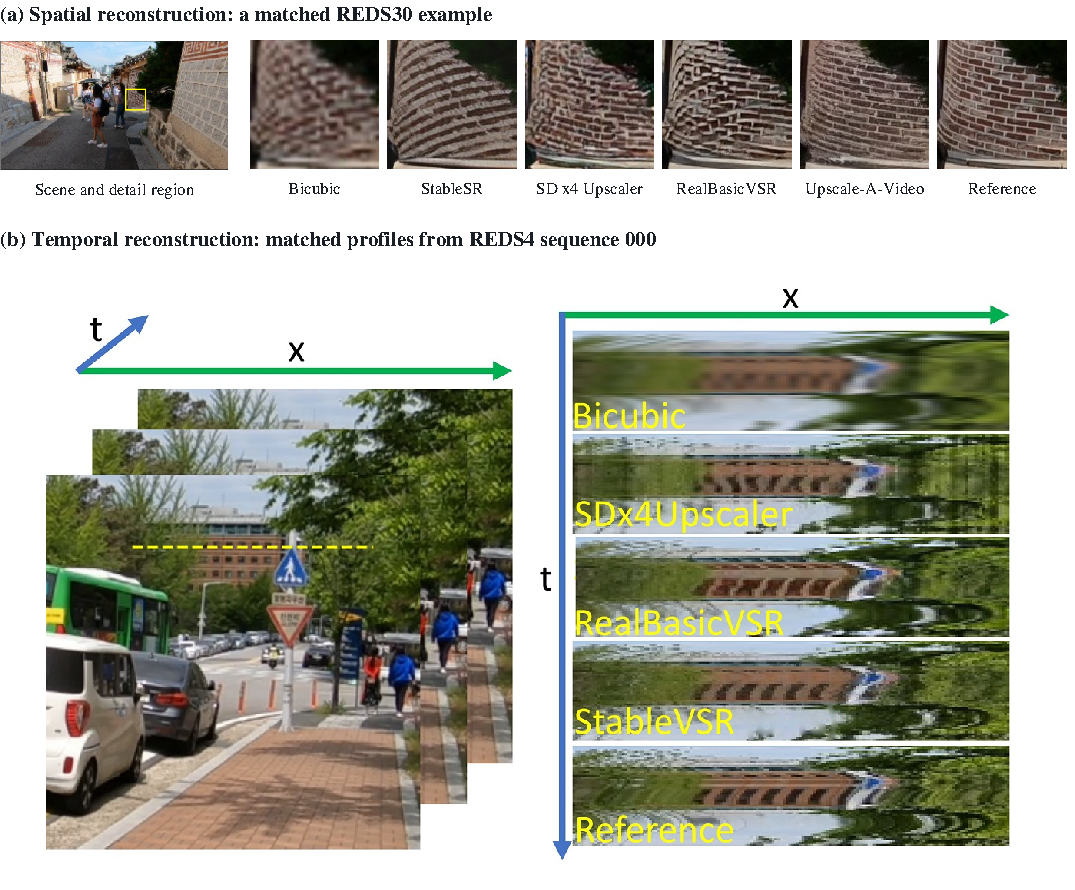
\includegraphics[width=\textwidth]{figures/tradeoff.pdf}
\caption{Published visual comparisons of spatial and temporal reconstruction. (a) Matched brick-wall crops from Upscale-A-Video~\cite{upscale}, Fig.~4, on REDS30: detail sharpness and agreement with the reference structure are different properties. The yellow box identifies the compared region. (b) Temporal profiles from StableVSR~\cite{stablevsr}, Fig.~6, on REDS4 sequence 000. Each profile stacks the same image row over time; horizontal position is $x$ and time runs downward. Irregular trajectories expose temporal artifacts.}
\label{fig:tradeoff}
\end{figure*}

Rapid changes in foundation models also complicate comparisons. Image diffusion models and video diffusion transformers differ in pretraining data, motion priors, model capacity, latent compression, and computational requirements. Restoration methods further vary in supervision, degradation simulation, temporal context, guidance, and sampling steps. A gain obtained with a stronger backbone can therefore reflect both a better prior and a better restoration mechanism. Meanwhile, one-step and streaming methods introduce new questions about first-frame latency, future-frame access, cache state, and the cost of encoding and decoding.

Evaluation must accommodate these changes. Reference-based distortion metrics measure agreement with a target, perceptual metrics assess appearance similarity, and no-reference predictors estimate viewing quality. None alone describes whether generated detail is faithful and temporally stable. Recent subjective evaluation of diffusion-based VSR shows that metric performance depends on the restoration method, source content, and aggregation protocol~\cite{metric}. Together with uneven task coverage, these issues motivate a survey that connects method design, application requirements, and evaluation.

Existing surveys provide complementary perspectives on this field. Li et al.~\cite{irsurvey} review diffusion-based image restoration through supervised and zero-shot formulations, conditioning strategies, and blind or real-world degradation. Jiang et al.~\cite{aiosurvey} organize all-in-one image restoration by network design, learning strategies, and techniques. These perspectives explain how restoration models acquire generality, but video additionally requires motion-aware processing and persistent content across frames. Xing et al.~\cite{videodiffsurvey} survey video diffusion models across generation, editing, and understanding. Their broad generative perspective provides foundations for temporal architectures and conditioning. Rota et al.~\cite{vrsurvey} review video restoration architectures, loss functions, and benchmarks, providing a detailed account of temporal information use. Building on these foundations, the present survey centers the interaction between diffusion priors and video reconstruction. Table~\ref{tab:surveys} summarizes the relationship between these lines of work.

\begin{table*}[t]
\caption{Representative surveys related to diffusion-based video restoration and enhancement.}
\label{tab:surveys}\centering\footnotesize
\begin{tabularx}{\textwidth}{@{}p{0.23\textwidth}YYY@{}}\toprule
Survey & Main focus & Principal organizing dimensions & Relation to video restoration \\\midrule
Diffusion image restoration~\cite{irsurvey} & Image reconstruction with diffusion models & Supervision, conditioning, generation space, real-world degradation & Establishes prior adaptation and inverse-problem formulations \\
All-in-one image restoration~\cite{aiosurvey} & Unified restoration across degradations & Architectures, learning, prompts, experts, multimodal and agentic systems & Motivates multi-task models and adaptive restoration systems \\
Video diffusion~\cite{videodiffsurvey} & Generation, editing, and video understanding & Generative architectures, conditions, applications & Provides spatiotemporal priors and includes restoration applications \\
Deep video restoration~\cite{vrsurvey} & Learning-based video reconstruction & Architecture, motion handling, losses, datasets & Establishes temporal modeling and task-specific evaluation \\
This survey & Diffusion-based video restoration and enhancement & Priors, conditioning, temporal mechanisms, tasks, efficiency, evaluation & Connects generative detail to source fidelity and temporal consistency \\\bottomrule
\end{tabularx}
\end{table*}

This survey covers methods that use diffusion, score-based, or related flow priors to restore a video, which spans spatial and spatiotemporal super-resolution, single and mixed degradation removal, domain-specific enhancement, and restoration of generated video. Our main contributions are as follows:
\begin{itemize}
\item We develop a unified taxonomy spanning degradation assumptions, learning strategies, prior sources, conditioning, temporal modeling, inference efficiency, and system organization.
\item We analyze how noise coupling, correspondence, propagation, attention, memory, and decoding connect generated detail to the input sequence, and compare the strengths and limitations of representative approaches.
\item We review restoration tasks across natural video and specialized domains, relating their imaging characteristics and temporal requirements to suitable generative models.
\item We examine datasets and evaluation metrics, discuss fair comparisons across heterogeneous backbones, and identify research directions in quality control, efficient long-video processing, and generalization.
\end{itemize}

Section~\ref{sec:formulation} introduces the background and problem formulation. Section~\ref{sec:methodology} reviews generative priors, conditioning, temporal modeling, learning strategies, and efficient inference. Section~\ref{sec:tasks} relates these mechanisms to restoration tasks and application domains. Section~\ref{sec:evaluation} discusses datasets, quality assessment, and fair comparisons, and Section~\ref{sec:outlook} identifies challenges and future directions.

\begin{figure*}[t]
\centering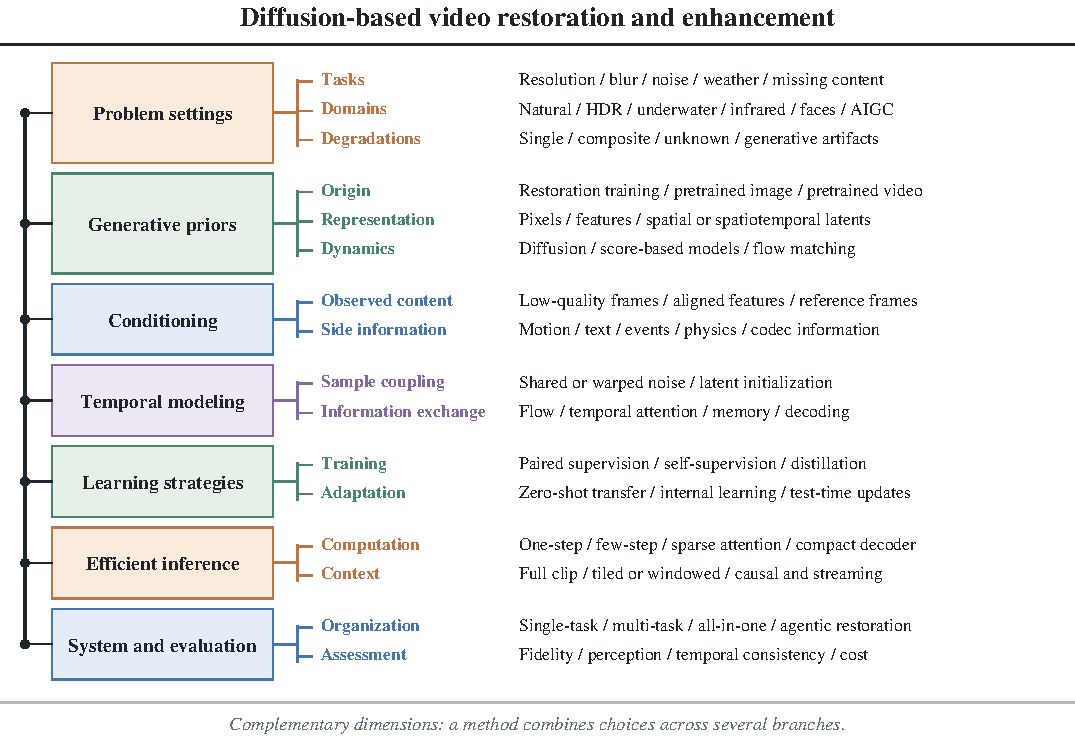
\includegraphics[width=\textwidth]{figures/taxonomy.pdf}
\caption{Taxonomy and organization of diffusion-based video restoration and enhancement. The classification connects task and degradation characteristics with generative priors, learning strategies, conditioning, temporal modeling, and inference.}
\label{fig:taxonomy}
\end{figure*}

\section{Background and Taxonomy}
\label{sec:formulation}
\subsection{Video Restoration and Enhancement}
Let $X=(x_1,\ldots,x_T)$ denote a clean or desired video and $Y=(y_1,\ldots,y_{T'})$ its observed counterpart. A general observation model is
\begin{equation}
Y=\mathcal{D}_{\phi}(X)+N,
\label{eq:observation}
\end{equation}
where $\mathcal{D}_{\phi}$ represents degradation parameterized by $\phi$ and $N$ denotes residual noise. The degradation can couple spatial resolution, motion, color, exposure, and compression, and its parameters may vary over time. Spatial VSR typically preserves the number of frames, whereas interpolation and spatiotemporal super-resolution have different input and output temporal sampling. Noise can depend on the signal, and operations such as compression are nonlinear.

Restoration seeks to recover information consistent with the underlying scene. Enhancement additionally concerns visibility, dynamic range, and perceptual appearance, including settings without a unique clean reference. This distinction is relevant to low-light and underwater processing, where appearance depends on illumination and rendering choices, and to generated-video enhancement, where artifacts may not follow a known physical degradation process. In both cases, the input provides structure and temporal context that constrain the desired output.

For a known degradation model, generative restoration can be interpreted through
\begin{equation}
p(X\mid Y,\phi,c)\propto p(Y\mid X,\phi,c)\,p_{\theta}(X\mid c),
\label{eq:posterior}
\end{equation}
assuming that the scene prior is independent of $\phi$ given auxiliary conditions $c$. These conditions may include reference frames, identity information, events, text, or acquisition metadata. The likelihood links the reconstructed video to its observation, while the prior models plausible content. In blind restoration, the degradation parameters may be estimated, marginalized, or handled implicitly by a conditional network. Practical diffusion restorers implement this interaction in different ways, including learned conditioning, approximate posterior guidance, and distilled prediction~\cite{ddrm,dps,seedvr2}.

\subsection{Restoration Objectives}
\textbf{Fidelity.} Fidelity concerns agreement with the underlying scene. With an aligned clean reference, it can be evaluated through a distance $d(\widehat X,X)$. Without such a reference, observation consistency, such as $\|\mathcal D_{\widehat\phi}(\widehat X)-Y\|$, tests whether the reconstruction explains the input. Observation consistency alone leaves ambiguity in detail lost during degradation, including null-space components in a linear model. Identity, geometry, text, and radiometry provide additional constraints in specialized applications.

\textbf{Perceptual quality.} Perceptual quality concerns the visual plausibility and viewing quality of the reconstructed video. A sharp texture may look natural while differing from the reference, particularly when fine detail has been removed. The perception--distortion tradeoff describes this tension between distributional realism and expected reconstruction error~\cite{perception_distortion}. Perceptual similarity to a particular reference and naturalness of an output are related but distinct evaluation objectives.

\textbf{Temporal consistency.} Temporal consistency requires appearance, structure, and identity to evolve in agreement with motion and visibility. Correctly restored frames may change substantially under camera motion, occlusion, or lighting changes. Consequently, temporal modeling must preserve meaningful changes while suppressing flicker, texture drift, and inconsistent reconstruction. A video prior supplies learned motion regularities, while observation-based correspondence ties those regularities to the particular sequence being restored~\cite{svd,upscale,stablevsr}.

These objectives interact with computational cost. The design problem can be expressed as
\begin{equation}
\min_{\mathcal A}\left(
\mathcal L_{\mathrm{fid}},\,
\mathcal L_{\mathrm{perc}},\,
\mathcal L_{\mathrm{temp}},\,
\mathcal C\right),
\label{eq:objectives}
\end{equation}
where $\mathcal A$ is the restoration procedure and $\mathcal C$ represents resource use. Different applications favor different operating points. Scientific or identity-sensitive video emphasizes faithful reconstruction, while entertainment enhancement may place greater weight on perceptual detail. Long-duration and interactive applications additionally constrain latency, memory, and temporal context.

\subsection{Taxonomy of Diffusion-Based Video Restoration}
\textbf{Tasks, domains, and degradations.} Super-resolution, denoising, deblurring, dehazing, and compression artifact reduction specify restoration tasks. Natural RGB, faces, underwater scenes, infrared, HDR, and generated video introduce distinct content or acquisition characteristics. Degradations can occur individually, in known combinations, or in open settings with unknown composition and severity. For example, turbulent infrared video may combine geometric distortion, blur, and limited resolution; a face video may contain noise, compression, and motion blur.

\textbf{Learning and degradation knowledge.} Paired supervision learns from degraded and clean examples; unpaired and self-supervised learning use alternative training signals. Blindness describes uncertainty about the corruption at inference. Zero-shot transfer concerns generalization to a target task, domain, or sequence without corresponding training. A supervised model can therefore be blind, and a training-free method can rely on a known observation operator. Table~\ref{tab:definitions} summarizes terminology used throughout the survey.

\textbf{Prior source and modeling space.} A generative prior may be learned for restoration, adapted from a pretrained image model, or inherited from a video foundation model. Pixel-space modeling operates directly on image intensities, while latent-space modeling uses a learned encoder and decoder to reduce dimensionality~\cite{ldm}. Diffusion and flow matching describe generative formulations; U-Nets and diffusion transformers describe architectures. Their combinations lead to different appearance priors, temporal capabilities, and computational costs.

\textbf{Conditioning and temporal mechanisms.} Observations can guide generation through direct input, feature adapters, reference frames, physical constraints, or sampling-time guidance. Temporal dependencies can be introduced through correlated noise, flow-based propagation, recurrent state, joint attention, or temporal decoding. These choices are complementary: an image prior can acquire temporal behavior through additional modules, while a video prior still benefits from explicit observation conditioning.

\textbf{Inference and system paradigms.} Iterative, few-step, and one-step models differ in the number of generative updates. Offline, windowed, and streaming processing differ in temporal access and state management. Single-task systems specialize in one restoration objective; multi-task and all-in-one models share representations across degradations. Routed and agentic systems coordinate several operators, potentially including both diffusion and conventional restoration models.

\begin{table}[t]
\caption{Terminology for learning, task coverage, and inference.}
\label{tab:definitions}\centering\footnotesize
\begin{tabularx}{\columnwidth}{@{}p{0.29\columnwidth}Y@{}}\toprule
Term & Meaning \\\midrule
Blind & Degradation parameters or types are unknown at inference. \\
Zero-shot & Transfer to a specified task, domain, or sequence without target-specific training. \\
Training-free & Reuse of learned model parameters without additional training; inference may still require optimization. \\
All-in-one & A unified model addresses multiple degradation types within a shared checkpoint. \\
One-step & Restoration uses one generative sampling update; auxiliary network costs can remain. \\
Streaming & Frames are processed incrementally with bounded look-ahead and maintained state. \\
Real-time & Processing keeps pace with the target frame rate under specified deployment conditions. \\\bottomrule
\end{tabularx}
\end{table}

Together, these dimensions support comparisons beyond task names or sampling steps. Two models that both perform blind VSR may differ substantially in their pretraining, supervision, temporal context, and use of side information. Conversely, methods for different tasks may share the same principle of coupling a strong visual prior to motion and measurement constraints.

\section{Methodology}
\label{sec:methodology}
Diffusion-based video restoration combines a generative prior with mechanisms that preserve observed content and temporal structure. This section reviews four complementary design choices: the source and conditioning of the prior, temporal information exchange, learning and system organization, and efficient inference. The same mechanisms recur across restoration tasks, while their relative importance depends on the degradation and available observations.
\subsection{Generative Priors and Conditioning}
\label{sec:priors}
\subsubsection{Diffusion and Score-Based Reconstruction}
For a clean video representation $Z_0$, the standard Gaussian forward process takes the form
\begin{equation}
Z_s=\sqrt{\bar\alpha_s}Z_0+\sqrt{1-\bar\alpha_s}\,\epsilon,
\quad \epsilon\sim\mathcal N(0,I),
\end{equation}
where $s$ indexes diffusion noise rather than video time. A denoiser learns to predict noise, the clean representation, or a related velocity parameterization. Conditional restoration typically trains a denoiser using the observation representation $c(Y)$:
\begin{equation}
\mathcal L_{\epsilon}=\E\!\left[\left\|\epsilon-\epsilon_\theta(Z_s,s,c(Y))\right\|_2^2\right].
\end{equation}
DDPM, DDIM, and continuous-time score formulations provide different training and sampling perspectives~\cite{ddpm,ddim,score_sde}. Their practical role in restoration depends on what is conditioned upon, where the state lives, and whether the model was trained to describe videos or individual images.

Posterior-guided approaches instead reuse a generative prior and incorporate the observation during inference~\cite{ddrm,dps}. In latent restoration, a common approximation applies a likelihood-related gradient through a predicted clean latent and its decoder:
\begin{equation}
g_s \approx -\nabla_{Z_s}\,\ell\!\left(Y,\mathcal D_{\phi}\bigl(D(\widehat Z_0(Z_s))\bigr)\right).
\label{eq:guidance}
\end{equation}
Here $D$ is the decoder, and $\ell$ is an observation discrepancy, not necessarily an exact negative log-likelihood. The quality of this approximation depends on the noise level and the accuracy of the predicted clean representation. Unknown degradations, nonlinear codecs, errors in $\widehat Z_0$, and lossy decoding can all weaken its connection to the desired posterior. For videos, a framewise likelihood also does not automatically impose a joint temporal prior.

\subsubsection{Sources of Generative Priors}
\textbf{Training for restoration.} A task-specific diffusion process can learn a compact restoration distribution without inheriting a large text-conditioned foundation model. VD-Diff, for example, combines wavelet-aware video modeling with a learned latent prior for deblurring~\cite{vddiff}. SeedVR extends restoration-specific learning to a video transformer, while SeedVR2 combines a restoration-trained teacher with distillation and adversarial post-training~\cite{seedvr,seedvr2}. This route offers control over training data and objectives, at the cost of learning the relevant visual and motion distributions.

\textbf{Pretrained image priors.} Image diffusion models provide detailed appearance knowledge and accessible initialization~\cite{ldm}. Upscale-A-Video and StableVSR adapt image super-resolution priors with video-specific conditioning~\cite{upscale,stablevsr}. MGLD-VSR guides a latent image prior with motion information~\cite{mgld}. ZVRD and DiffIR2VR-Zero investigate transferring image priors to video without additional video-task training~\cite{zvrd,diffir2vr}. The attraction is reuse, but the missing temporal distribution must be supplied through learned modules, correspondence, sampling constraints, or a combination of these mechanisms.

\textbf{Pretrained video priors.} Video diffusion models incorporate learned spatial and temporal dependencies~\cite{svd,wan}. Their motion prior can reduce the burden on externally imposed frame coupling. Nevertheless, a model trained to generate plausible motion need not preserve the exact motion in a degraded observation. STAR uses a text-to-video foundation to support real-world VSR, DOVE adapts a video prior for efficient one-step restoration, and SVD-based methods such as DC-VSR expose the role of attention propagation across spatial and temporal partitions~\cite{star,dove,dcvsr}. The inherited motion prior reduces the amount of temporal structure that must be learned from restoration pairs, although the low-quality observation remains essential for preserving the particular motion of the input.

\textbf{Diffusion-derived representations.} A diffusion model can contribute useful representations even when the final enhancement network does not run a reverse-diffusion chain. UnDIVE transfers an encoder learned by generative pretraining into a physics-based underwater enhancement system~\cite{undive}. This use of diffusion separates representation learning from generative inference: the deployed enhancement network benefits from pretraining without executing a reverse-diffusion chain.

The amount and location of adaptation also matter when comparing pretrained video priors. LiteVSR freezes the Wan2.2-5B transformer and trains a state-aware dual-stream adapter with a lightweight fusion layer, retaining a flow-matching objective in latent space~\cite{litevsr}. Its implementation explicitly excludes pixel-domain losses, and the default evaluation uses five UniPC steps; single-step sampling is an additional supported operating point rather than the sole definition of the method. This differs from pipelines that retrain the decoder or introduce adversarial supervision after an initial latent-space stage. The division between frozen and trainable components determines both data requirements and how strongly restoration training can alter the pretrained distribution.

\subsubsection{Pixel, Feature, and Latent Representations}
Pixel-space modeling keeps the output variables close to the observation model but exposes the denoiser to the full spatial and temporal resolution. Latent diffusion reduces this cost with an encoder $E$ and decoder $D$~\cite{ldm}. Restoration then depends on both the generative model and the autoencoder's ability to preserve information. Fine text, edges, thermal structures, or small moving objects may be lost before denoising, while a framewise decoder can reintroduce flicker into a coherent latent sequence.

Spatial and temporal compression affect reconstruction in different ways. A video autoencoder with temporal compression changes the correspondence between input frames and latent tokens; treating it as a drop-in image encoder can create alignment or boundary errors. MGLD-VSR explicitly addresses temporal behavior in decoding, whereas recent efficient methods redesign or condition the decoder to reduce both cost and reconstruction loss~\cite{mgld,flash,swiftvr}. The autoencoder thus sets a representation ceiling: detail discarded during encoding or destabilized during decoding cannot be attributed solely to the denoising model.

\subsubsection{Flow Matching and Distilled Generators}
Flow matching and rectified flow learn a vector field that transports a base distribution toward a data distribution~\cite{rectifiedflow,sd3}. For a simple straight interpolation $Z_\tau=(1-\tau)\epsilon+\tau Z_0$, one illustrative objective is
\begin{equation}
\mathcal L_{\mathrm{FM}}=\E\left[\left\|v_\theta(Z_\tau,\tau,c)-(Z_0-\epsilon)\right\|_2^2\right].
\end{equation}
Inference integrates $dZ_\tau/d\tau=v_\theta(Z_\tau,\tau,c)$. This family is connected to diffusion through continuous-time generative modeling, with a distinct training path and prediction target. UniFlowRestore is an example of flow-based restoration rather than a conventional DDPM formulation~\cite{uniflowrestore}. The terminology is particularly relevant for newer video backbones and distilled restoration models.

One-step restoration may arise from teacher--student distillation, direct adaptation of a pretrained one-step model, adversarial post-training, or task-specific training. A one-step student does not retain all the iterative correction opportunities of its teacher. The training objective must absorb observation fidelity, detail generation, and temporal regularity into a single evaluation. DOVE, DLoRAL, and SeedVR2 use different routes to this goal~\cite{dove,dloral,seedvr2}; grouping them by step count alone conceals their distinct priors and training costs.

\begin{figure*}[t]
\centering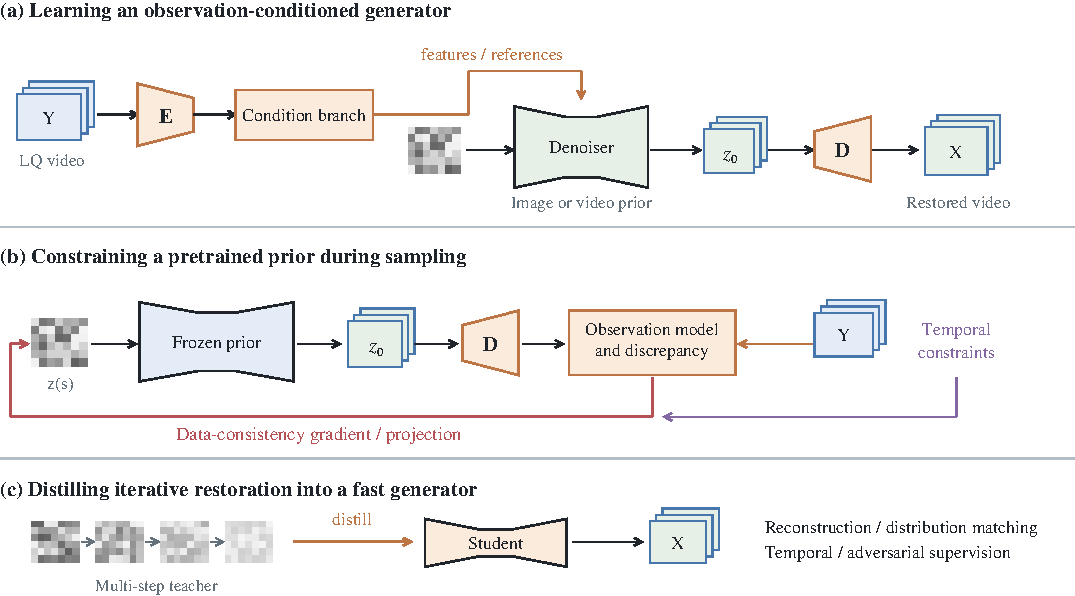
\includegraphics[width=\textwidth]{figures/prior_routes.pdf}
\caption{Three ways to connect a generative prior to video observations. (a) A learned condition branch guides denoising. (b) Observation discrepancy and temporal constraints refine sampling with a pretrained prior. (c) Distillation transfers an iterative teacher to a fast student. $E$ and $D$ denote the encoder and decoder; $Y$ and $X$ denote observed and reconstructed videos.}
\label{fig:routes}
\end{figure*}

\subsubsection{Observation and Multimodal Conditioning}
Figure~\ref{fig:routes} separates the point at which restoration evidence enters the generative process. Direct concatenation, adapters, and ControlNet-style branches feed low-quality observations into intermediate features. Observation gradients and projection-like updates act during sampling. Reference frames supply appearance or identity evidence, while optical flow, events, codec metadata, and physical image-formation models add information that an RGB-only prior may not recover reliably~\cite{cpgdnet,flair,undive,diqp}.

Text can specify a desired appearance or identify a degradation, but it usually contains less geometric evidence than the observed frames. A prompt such as ``sharp detailed face'' cannot resolve the identity of a heavily blurred person. The spatial observation therefore remains necessary even when semantic guidance improves texture generation. Similarly, strong classifier-free or task guidance can alter the balance between prior and observation, but increasing its scale is not guaranteed to improve all three quality objectives. Guidance schedules determine when semantic information shapes appearance and when observations dominate structural reconstruction.

Physical and semantic conditions can also conflict. A reference portrait may provide an identity while differing in pose, age, illumination, or expression. Codec motion vectors are useful side information but are optimized for rate--distortion coding rather than exact optical flow. Events reveal brightness changes but do not directly encode absolute radiance. Good conditioning uses each signal within its domain of validity and leaves room for uncertainty when the signals disagree.

Conditioning should be matched to the spatial and temporal support of the denoising computation. Tiled Prompts identifies a mismatch between a global caption and local latent tiles: a global description can omit a small object or impose content that is irrelevant to a particular region~\cite{tiledprompts}. It supplies local captions to image tiles or video tubes as an inference-time modification of existing super-resolution systems; the main video experiments use STAR with an I2VGen-XL backbone. Sparse visual references offer a complementary form of control. SparkVSR propagates high-resolution keyframes through a CogVideoX1.5-5B image-to-video prior while anchoring motion to the low-resolution sequence, with latent-then-pixel training and reference-free guidance~\cite{sparkvsr}. Textual and visual references thus provide different controls: local prompts constrain semantic relevance, whereas keyframes supply explicit appearance that can be propagated through the sequence.

\subsection{Temporal Modeling}
\label{sec:temporal}
Temporal consistency is not the requirement that adjacent frames look alike. It requires that changes agree with motion, occlusion, illumination, and scene structure. A static-background assumption can be useful in one region and wrong in another. A model must preserve actual motion while suppressing unexplained appearance changes. Figure~\ref{fig:temporal} shows how two representative systems implement this requirement. StableVSR obtains texture guidance from a motion-compensated neighboring reconstruction, whereas Upscale-A-Video combines local temporal modules, recurrent propagation across segments, and temporal decoding. The location and reach of information exchange determine which temporal errors each design can address.

\begin{figure*}[t]
\centering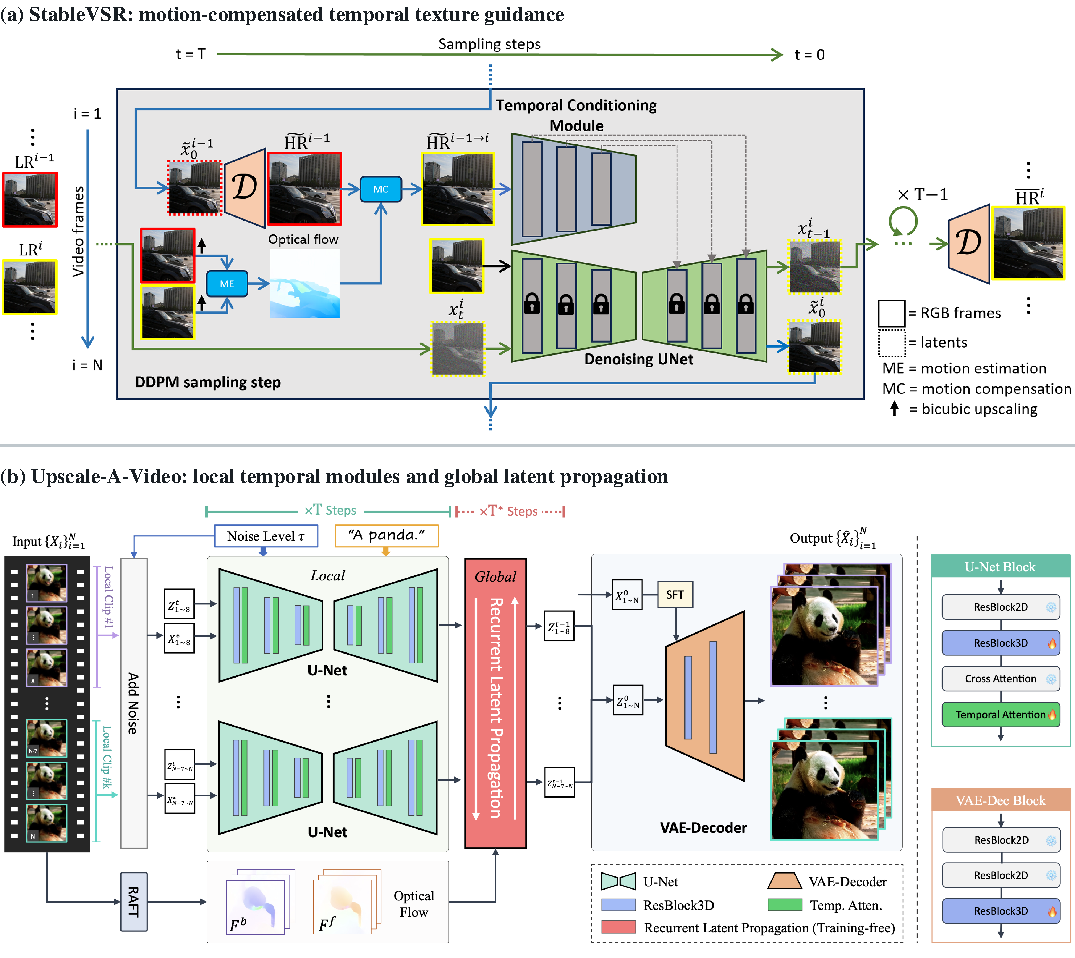
\includegraphics[width=\textwidth]{figures/temporal_mechanisms.pdf}
\caption{Concrete architectures for temporal modeling, reproduced from the original papers under \href{https://creativecommons.org/licenses/by/4.0/}{CC BY 4.0}. (a) StableVSR~\cite{stablevsr}, Fig.~2: optical flow warps reconstructed texture from a neighboring frame, and a temporal conditioning module guides the frozen denoising U-Net. (b) Upscale-A-Video~\cite{upscale}, Fig.~2: temporal layers model local clips, bidirectional recurrent latent propagation exchanges information across clips at selected diffusion steps, and a finetuned VAE decoder improves RGB consistency. Original module names and frozen/trainable annotations are retained.}
\label{fig:temporal}
\end{figure*}

\subsubsection{Noise Coupling and Initialization}
Independent framewise sampling allows each frame to choose a different plausible explanation of missing texture. Sharing, correlating, or propagating initial noise reduces this source of variation~\cite{zvrd}. However, identical image-coordinate noise is not identical object-coordinate noise when the camera or object moves. A texture can remain fixed to the screen rather than to a surface. Motion-aware noise propagation is a more appropriate conceptual target, but resampling changes noise statistics and requires a policy for disoccluded regions.

Initialization also controls how much a video changes. Noise Calibration constrains the starting noise of a pretrained video diffusion model to preserve source content~\cite{ncsdedit}. Inpainting methods can initialize from a coarse, temporally coherent completion rather than pure noise~\cite{diffueraser}. These choices restrict the space explored by the generator, but they can also preserve errors in the initialization. The relevant question is not merely whether frames become more similar; it is whether the initialization supports correct detail and motion after refinement.

Warped Diffusion~\cite{warped} first adapts SDXL to conditional image restoration, including training with correlated Gaussian-process noise. It then warps a continuous noise field according to motion and uses inference-time equivariance self-guidance to align denoiser predictions across frames. Its central insight is that correlated inputs alone do not guarantee correlated outputs: the denoiser must also behave consistently under the corresponding transformation. The resulting model transfers image restoration knowledge to video without learning from video training pairs.

\subsubsection{Correspondence and Motion-Guided Propagation}
Given estimated correspondence $u_{t-1\rightarrow t}$ and an occlusion-validity mask $M_t$, a typical temporal penalty is
\begin{equation}
\mathcal L_{\mathrm{warp}}=
\frac{\sum_t\|M_t\odot[\widehat x_t-\mathcal W(\widehat x_{t-1},u_{t-1\rightarrow t})]\|_1}
{\sum_t\|M_t\|_1+\varepsilon},
\label{eq:warp}
\end{equation}
where $\mathcal W$ warps a preceding frame into the current coordinates. Related constraints can act on features or latents rather than RGB output. Upscale-A-Video combines temporal modules with flow-guided latent propagation; StableVSR uses temporal conditioning and texture guidance; MGLD-VSR introduces motion guidance into the diffusion trajectory~\cite{upscale,stablevsr,mgld}. DiffIR2VR-Zero transfers information with hierarchical latent warping and token merging~\cite{diffir2vr}.

These approaches use observed redundancy to constrain ambiguity, but correspondence is least reliable precisely where restoration is hardest: heavy blur, low light, rain, repetitive texture, large motion, and occlusion. Warping a wrong texture consistently can improve a temporal score while reducing fidelity. Confidence weighting and disocclusion handling are therefore central, not minor implementation details. At motion boundaries, the flow estimator and restoration model interact: improving propagation requires both accurate correspondence and protection against invalid matches.

Long-range propagation adds a second failure mode. Information reused across many frames can preserve identity through temporary occlusion, but an early hallucination can also become persistent state. Local coherence is not evidence of globally correct reconstruction. Scene-cut resets, confidence-weighted updates, and re-anchoring to current observations can limit error accumulation over long clips.

Temporal consistency depends on which information is propagated and where it enters the restoration process. Dense motion alignment, instance-level semantics, and learned video dynamics provide different forms of temporal support. DGAF-VSR revisits feature compensation inside a diffusion pipeline: its Optical Guided Warping Module aligns features through an upscale--warp--downscale operation, while its Feature-wise Temporal Condition Module supplies dense guidance from neighboring frames~\cite{dgaf}. This design seeks to preserve useful high-frequency evidence before the generative model supplies missing detail; the reported benefit of increasing the warping resolution is not monotonic. Semantic correspondence offers another route when local appearance is unreliable. SeeClear couples instance-centric clip alignment and a channel-wise texture memory with a frozen OpenSeeD semantic distiller~\cite{seeclear}. Its blurring ResShift process operates on discrete-wavelet subbands, avoiding a learned autoencoder; the DCT-based blur construction and DWT-based representation serve distinct purposes. SeTe-VSR instead injects SAM2 semantic embeddings and temporal-spatial awareness into an SD2.1-based latent denoiser and augments the VAE decoder with temporal layers~\cite{setevsr}. These approaches illustrate that temporal support can reside in aligned observations, object-level representations, or the reconstruction decoder. The resulting mechanisms address different failure modes: flow alignment depends on correspondence accuracy, semantic alignment depends on object representations, and decoder adaptation targets the conversion of coherent features into stable pixels.

\subsubsection{Temporal Layers, Attention, and Memory}
Learned temporal convolution, recurrent modules, state-space components, and temporal attention allow features from multiple frames to influence denoising. These mechanisms can be trained as additions to an image prior or inherited from a video prior~\cite{upscale,scst,star}. The distinction affects both data requirements and the source of improvement. An added temporal block learns motion from restoration data, whereas a video foundation model has already absorbed a motion distribution during pretraining.

Attention supports interaction beyond explicit flow, but it does not guarantee correct correspondence. Similar-looking regions may exchange incompatible details, and global attention can become expensive at high spatial and temporal resolution. Windowed attention limits cost but introduces a new requirement: information must cross window boundaries in a controlled way. SeedVR's shifted variable-size windows and DC-VSR's spatial and temporal attention propagation exemplify mechanisms for extending processing beyond the native support of a backbone~\cite{seedvr,dcvsr}.

Memory and cached keys/values can preserve context while reducing repeated computation. Their correctness depends on how cached features align with the current denoising state and frame positions. A cache designed for autoregressive synthesis cannot be assumed to preserve restoration fidelity under arbitrary input changes. Streaming VSR methods consequently combine cache or propagation strategies with observation-conditioned restoration~\cite{stream,infvsr,flash}. Their central difficulty is keeping cached context useful under accumulated drift, abrupt motion, and scene transitions.

\subsubsection{Losses and the Decoder}
Temporal losses may act on warped RGB frames, deep features, motion-compensated residuals, or discriminator features. They encourage different invariances. A pixel penalty strongly preserves aligned intensities but may penalize true lighting change; a feature penalty can tolerate some appearance variation but miss fine flicker. An adversarial temporal loss can promote plausible dynamics without ensuring that those dynamics match the observed scene. No single loss should be equated with complete temporal correctness.

The decoder is a separate source of temporal error. Consistent latents can produce unstable high-frequency RGB detail if decoded independently. Temporal-aware decoding in MGLD-VSR and conditional or lightweight decoding in efficient methods make this issue explicit~\cite{mgld,flash}. This creates a second temporal modeling stage after denoising. Its interaction with spatial tiling and temporal chunking becomes particularly important when high-resolution videos exceed the decoder's native processing window.

\subsubsection{Comparison of Temporal Mechanisms}
\begin{table*}[t]
\caption{Comparison of temporal mechanisms, the information they constrain, and their characteristic challenges.}
\label{tab:temporal}\centering\footnotesize
\begin{tabularx}{\textwidth}{@{}p{0.18\textwidth}YYY@{}}\toprule
Mechanism & Representative use & What it constrains & Main challenge \\\midrule
Shared or calibrated noise & ZVRD; Noise Calibration~\cite{zvrd,ncsdedit} & Random variation or initial deviation from the source & Moving textures; scene cuts; several random seeds \\
Flow/latent propagation & Upscale-A-Video; MGLD-VSR; DiffIR2VR-Zero~\cite{upscale,mgld,diffir2vr} & Appearance along estimated correspondences & Disocclusion; incorrect flow; large motion; repetitive patterns \\
Temporal conditioning & StableVSR; FLAIR~\cite{stablevsr,flair} & Cross-frame feature and texture relationships & Long occlusion; identity changes; frame-rate shifts \\
Joint/windowed attention & STAR; SeedVR; DC-VSR~\cite{star,seedvr,dcvsr} & Contextual dependencies across frames or partitions & Window boundaries; native-context overflow; persistent objects \\
State/cache reuse & Stream-DiffVSR; InfVSR~\cite{stream,infvsr} & Recurrent context under bounded computation & Long-horizon drift; stale state; abrupt content change \\
Temporal decoding & MGLD-VSR; FlashVSR~\cite{mgld,flash} & Mapping from latent consistency to RGB consistency & Fine textures; tiled decoding; chunk boundaries \\\bottomrule
\end{tabularx}
\end{table*}

Table~\ref{tab:temporal} reveals complementary roles for these mechanisms. Noise coupling limits stochastic variation before reconstruction, while correspondence constrains geometric consistency along visible trajectories. Attention aggregates evidence beyond explicit pairwise warps, and memory extends that evidence over longer intervals. Temporal decoding then preserves the resulting latent consistency in pixel space. Combining these mechanisms can address different sources of flicker, but their errors can also interact: unreliable flow can contaminate memory, and an incoherent decoder can erase gains made by the denoiser.

\subsection{Learning Regimes and Restoration Systems}
\label{sec:learning}
\subsubsection{Paired, Self-Supervised, and Mixed Supervision}
The availability of training data determines how a restoration model connects its generative prior to degraded observations. Paired learning directly supervises this connection using degraded and clean videos. Because accurately aligned real pairs are difficult to acquire, synthetic degradation remains an important source of training data. It provides scalable supervision and precise control over corruption severity, but its effectiveness depends on how closely the simulated process represents real acquisition. A diffusion model trained on a narrow degradation distribution may reconstruct familiar inputs accurately while relying excessively on its prior when the observation falls outside that distribution.

For video, the degradation distribution has a temporal dimension. Independently sampling a corruption for each frame produces different statistics from persistent sensor noise or the periodic structure of a video codec. Mixed-degradation training further involves interactions among corruption types, strengths, and processing order. Noise followed by compression, for example, produces a different observation from compression followed by noise. Consequently, generalization concerns both unfamiliar individual degradations and unfamiliar combinations or temporal patterns of otherwise familiar degradations.

Self-supervision can complement paired learning at different stages of the restoration pipeline. SCST learns degradation-insensitive control features through a self-supervised objective within a broader paired VSR pipeline~\cite{scst}. UnDIVE combines unlabeled diffusion pretraining, paired spatial enhancement, and an unsupervised temporal constraint~\cite{undive}. These methods illustrate a hybrid learning regime in which prior learning, spatial reconstruction, and temporal regularization draw on different forms of supervision. Describing supervision at the component level therefore provides a more informative account of data requirements than assigning a single supervised or unsupervised label to the entire system.

InstantViR~\cite{instantvir} distills a pretrained video prior into a feed-forward inverse solver using degraded measurements and a known forward operator, without external clean/degraded training pairs. A measurement-likelihood term constrains fidelity while the frozen teacher regularizes the solution distribution. The solver uses bidirectional attention within each temporal block and causal attention with cached keys and values across blocks; its streaming claim therefore includes block buffering. LeanVAE reduces reconstruction overhead, with teacher-space regularization compensating for the change of latent representation during training. This connects generative distillation to blockwise streaming reconstruction.

\subsubsection{Zero-Shot Transfer and Test-Time Adaptation}
Zero-shot restoration encompasses several forms of transfer: applying an image restoration model to video, using a general generative prior with a new degradation operator, and restoring an unseen domain without paired target-domain training. ZVRD and DiffIR2VR-Zero exemplify image-to-video transfer~\cite{zvrd,diffir2vr}. Their relevance lies in reusing spatial restoration knowledge while introducing temporal coupling at inference. Zero-shot transfer does not necessarily eliminate auxiliary information: optical flow, pretrained restoration modules, estimated degradation parameters, and test-time optimization can still play substantial roles.

Test-time adaptation addresses distribution shift by updating model parameters from the observed test video. It differs from optimizing latent variables or initial noise while keeping the model fixed. Diffusion test-time adaptation for adverse weather combines a diffusion formulation with temporal calibration~\cite{difftta}. Such adaptation offers a way to exploit sequence-specific information, although its effectiveness depends on the amount and reliability of the available observations. Short sequences, abrupt scene changes, and severely corrupted frames can weaken the adaptation signal, while access to future frames changes whether a method is suitable for online processing.

These distinctions also clarify the computational implications of training-free inference. A frozen model may still require many gradient evaluations to optimize its input noise or latent representation. Conversely, a small parameter update can provide inexpensive sequence-specific calibration. The practical difference between these approaches thus involves the variables being optimized, the available temporal context, and the additional inference cost, rather than the presence or absence of offline training alone.

Temporal-Consistent Video Restoration~\cite{tcvr} instead treats the full reverse diffusion map as a differentiable generator and optimizes a shared seed and frame-dependent residuals under a MAP objective. Semantic structure in seed space and progressive optical-flow warping address consistency at different levels. Its four reverse steps describe the inner generator; the reported reconstruction still involves thousands of outer optimization iterations. The short inner chain makes differentiation through the complete generator tractable.

Domain-adaptive Video Deblurring via Test-time Blurring~\cite{dadeblur} uses diffusion to synthesize degradation rather than directly restore the test video. Relatively sharp patches are extracted from the target domain, and a pre-existing ID-Blau blur generator produces domain-matched pseudo training pairs that adapt a separate deblurrer. The resulting DADeblur framework uses generative modeling to improve the training distribution of a conventional restorer. Diffusion generates adaptation data at test time; after adaptation, the separate deblurring network restores frames without a reverse-diffusion chain for each output.

\subsubsection{Single-Task, Multi-Task, and All-in-One Models}
Single-task restoration allows the observation encoder, degradation model, and training objective to specialize in one problem. Multi-task learning shares representations across problems, while all-in-one restoration aims to handle multiple degradations with a common model, often through degradation prompts or shared conditional features. This distinction is particularly relevant when one architecture is trained into several task-specific checkpoints: architectural reuse provides less operational unification than a single checkpoint that handles all supported tasks. TDM and generic restoration models such as SeedVR illustrate the move toward broader task coverage~\cite{tdm,seedvr}; UniFlowRestore pursues a related objective through flow matching~\cite{uniflowrestore}.

Task diversity introduces interactions that cannot be inferred from performance on isolated degradations. Denoising may remove detail useful for subsequent deblurring, whereas deblurring may amplify residual noise. A model that handles each task independently therefore does not necessarily handle their composition. Open-degradation restoration extends this difficulty to corruption types and combinations absent from training. In this setting, identifying the degradation and estimating the reliability of the observation become closely connected to controlling the strength of generative correction.

Video adds a further interaction between task identification and temporal consistency. If degradation representations or routing decisions fluctuate across adjacent frames, restoration behavior can change even when the underlying scene remains stable. Temporally coherent conditioning helps avoid such discontinuities, but excessive persistence can delay adaptation to genuine changes in illumination, acquisition conditions, or scene content. Unified video restoration consequently requires both shared spatial restoration capability and appropriate temporal behavior in its degradation representation.

\subsubsection{Agentic and Routed Restoration}
Agentic restoration extends unification from a single model to a collection of tools. MoA-VR and VQ-Jarvis investigate systems that identify degradations, select or compose restoration operations, and assess output quality~\cite{moavr,vqjarvis}. Such systems can integrate diffusion models with regression networks, interpolation, compression, and quality estimation. Their relevance to diffusion-based restoration is therefore at the level of orchestration; diffusion need not be the mechanism of every component.

The effectiveness of orchestration depends jointly on the available specialists and the policy that selects them. Comparisons with a fixed operator or a fixed processing sequence help distinguish the contribution of adaptive routing from the strength of the tool library. An oracle selection provides an additional reference when the candidate outputs can be evaluated reliably. Tool calls and cumulative processing cost are also central to this system paradigm because repeated assessment and refinement can substantially increase latency.

Quality feedback creates a connection between restoration agents and the evaluation issues discussed in Section~\ref{sec:evaluation}. A judge that favors sharpness may encourage repeated enhancement and accumulate halos or unsupported texture; a judge that favors temporal smoothness may suppress genuine motion. Evidence preservation, stopping criteria, and recovery from harmful intermediate operations are therefore important research problems for agentic video restoration. They connect the choice of restoration tools to the reliability of the quality model that guides their use.

\subsection{Efficient Inference and Long-Video Processing}
\label{sec:efficiency}
\subsubsection{One-Step and Few-Step Restoration}
For a latent restoration pipeline, an approximate inference decomposition is
\begin{equation}
\begin{split}
\mathcal C_{\mathrm{total}}={}&\mathcal C_{\mathrm{encode}}
+\sum_{i=1}^{N_{\mathrm{FE}}}\mathcal C_{\mathrm{denoise},i}
+\mathcal C_{\mathrm{decode}}\\
&+\mathcal C_{\mathrm{aux}}+\mathcal C_{\mathrm{stitch}}.
\end{split}
\label{eq:cost}
\end{equation}
$N_{\mathrm{FE}}$ counts actual denoiser evaluations, including extra calls used by guidance when applicable, and $\mathcal C_{\mathrm{denoise},i}$ allows different costs for base and draft networks. The auxiliary term covers predictors, flow estimation, reference processing, and additional optimization outside these calls; the remaining terms cover autoencoding and spatial/temporal assembly. This decomposition explains why reducing sampling steps does not translate directly into an equal end-to-end speedup: encoding, decoding, and condition processing can dominate once repeated denoising becomes cheap. Parallel execution further affects the relationship between computation and latency.

One-step methods attack the repeated-denoising term. DOVE uses latent-pixel training, DLoRAL separates consistency and detail adaptation, UltraVSR combines one-step reconstruction with temporal mechanisms, and OS-DiffVSR uses multi-frame fusion and adjacent-frame adversarial training~\cite{dove,dloral,ultra,osdiff}. SeedVR2 uses distillation and adversarial post-training for generic restoration~\cite{seedvr2}. Their training objectives absorb detail synthesis, observation fidelity, and temporal regularity into a small number of evaluations, shifting computational effort from inference to adaptation or distillation.

Distillation must retain temporal behavior as well as single-frame realism. DUO-VSR progressively compresses a multistep teacher, then combines distribution matching with adversarial features from real and fake score models before preference-guided refinement~\cite{duovsr}. Its teacher is based on an internal 1.3B text-to-video model. AdcVSR transfers a DOVE teacher into a pruned SD2.1-based student with lightweight one-dimensional temporal convolutions~\cite{adcvsr}. Its pixel and feature discriminators each separate detail assessment from consistency assessment, making the potential conflict between these objectives explicit in the supervision. InstaVSR also uses a pruned image-diffusion backbone, but combines latent- and pixel-space adversarial learning with recurrent training and flow-guided temporal regularization~\cite{instavsr}. The latter predicts an output frame from five input frames, combining local multi-frame evidence with recurrent temporal supervision. These methods support a useful distinction between inheriting temporal structure from a video teacher, adding temporal computation to the student, and imposing temporal supervision during training.

Intermediate designs preserve selective refinement instead of forcing all restoration into one identical model evaluation. PS-SR assigns global reconstruction to one expensive base-model prediction and high-frequency refinement to a pruned draft model~\cite{pssr}. Its default four-stage configuration comprises one base evaluation and three draft evaluations, and the frequency-restricted update helps retain the low-frequency anchor. The term pseudo-single-step therefore describes an asymmetric computational budget rather than a single total function evaluation. SATB-VR takes a different approach: an auxiliary predictor initializes a higher-SNR state, SNR-aware trajectory blending trains the denoiser to tolerate prediction error, and denoiser-driven feature consistency improves the predictor~\cite{satbvr}. Its flexible few-step schedule preserves opportunities for correcting the initial estimate. These approaches retain selective correction after initialization, trading a small amount of additional computation for greater flexibility than a direct prediction. Table~\ref{tab:efficiency} summarizes complementary approaches to reducing computation. The number of generative updates, the cost of each update, and the amount of temporal buffering define different aspects of efficiency.

\begin{table*}[t]
\caption{Representative acceleration strategies. Sampling counts refer to the cited configurations; auxiliary prediction, encoding, decoding, and temporal buffering remain part of the complete system.}
\label{tab:efficiency}\centering\footnotesize
\begin{tabularx}{\textwidth}{@{}p{0.15\textwidth}p{0.16\textwidth}YY@{}}\toprule
Method & Generative updates & Principal cost reduction & Remaining computation / context \\\midrule
DOVE~\cite{dove} & One & One-step adaptation with latent-then-pixel training & Video DiT and autoencoder; joint clip context \\
TurboVSR~\cite{turbo} & Four-step setting & Highly compressed tokens and nonuniform shortcut learning & Spatiotemporal autoencoder and factorized conditioning \\
PS-SR~\cite{pssr} & One base + three draft & Expensive structure prediction followed by lightweight refinement & Four network evaluations of unequal cost \\
FastVSR~\cite{fastvsr} & One & Asymmetric encoder/decoder and compressed denoising grid & Spatial expansion and detail reconstruction in the decoder \\
AdcVSR~\cite{adcvsr} & One & Pruned image-prior student with lightweight temporal layers & Multi-frame processing; distillation from DOVE \\
OASIS~\cite{oasis} & One & Specialized attention and replacement of the VAE encoder & Video denoiser and decoder; learned input projection \\
InstantViR~\cite{instantvir} & Feedforward solver & Amortized inference, cached state and LeanVAE & Bidirectional context within each buffered block \\
SATB-VR~\cite{satbvr} & One--ten-step schedules & High-SNR initialization and trajectory blending & Auxiliary predictor plus selected denoising updates \\\bottomrule
\end{tabularx}
\end{table*}

\subsubsection{Representation and Network Compression}
Reducing denoiser evaluations is only one route to lower latency. TurboVSR reduces the number of tokens through an LTX autoencoder with $32\times32\times8$ compression, factorizes first-frame and remaining-frame conditioning, and converts the denoiser to a nonuniform shortcut model with a four-step operating point~\cite{turbo}. FastVSR instead changes the autoencoder interface: an asymmetric $f8$ encoder and $f16$ decoder permit a smaller denoising representation, with spatial expansion deferred to decoding and lower-bound-guided training used to stabilize the decoder~\cite{fastvsr}. OASIS removes further computation through attention-head specialization, replaces the VAE encoder with pixel unshuffle and linear projection, and progressively trains on temporally consistent and then inconsistent degradations~\cite{oasis}. Together, these designs show why step count is an incomplete cost measure. Token resolution, temporal compression, attention structure, and autoencoding jointly determine the end-to-end computational cost. High compression may reduce the computational burden while changing the evidence available for fine detail and motion reconstruction.

\subsubsection{Spatial Tiling and Temporal Windows}
At high resolution, memory may be dominated by latent features, attention activations, or decoding. Spatial tiling reduces peak memory but removes context and introduces stitching boundaries. PatchVSR and DC-VSR explicitly exchange information beyond isolated patches~\cite{patch,dcvsr}. Tile dimensions, overlap, and blending determine how much boundary context is retained. Global information from the full input can reduce semantic disagreement between tiles.

Temporal windows face a similar tradeoff. Overlapping clips provide local bidirectional context but repeat computation and may yield inconsistent boundary frames. Variable-size or shifted windows, as in SeedVR, address context management inside the model~\cite{seedvr}. External window blending can hide discontinuities without solving global identity drift. Boundary artifacts can consequently remain even when the interior of each clip is restored well.

\begin{figure*}[t]
\centering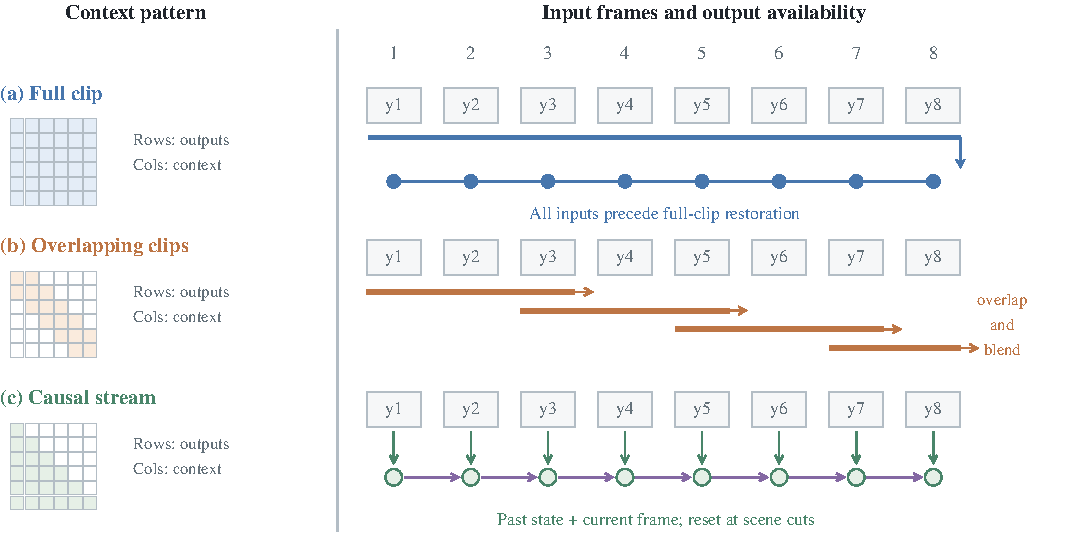
\includegraphics[width=\textwidth]{figures/deployment.pdf}
\caption{Temporal context in full-clip, overlapping-window, and causal inference. The matrices show allowed context interactions; the right-hand diagrams illustrate frame access and propagation. Full-clip processing uses future frames, overlapping windows reuse local context, and causal streaming carries state from past observations.}
\label{fig:deployment}
\end{figure*}

\subsubsection{Causality, Throughput, and Latency}
Figure~\ref{fig:deployment} distinguishes full-clip processing, overlapping windows, and causal streaming. Throughput measures sustained output rate; latency measures the delay experienced by an input frame or by the first output. A method can process a completed clip quickly while requiring the entire clip in advance. It can also have high steady-state throughput while buffering several future frames.

Stream-DiffVSR uses a four-step, frame-causal process with motion-aligned autoregressive guidance and temporal decoding~\cite{stream}. Its initialization descends from the StableVSR upscaler lineage. FlashVSR combines one-step inference, sparse attention, and a compact conditional decoder, while InfVSR uses causal transformer processing with a rolling cache~\cite{flash,infvsr}. Chunk-oriented streaming can introduce future-frame waiting within a chunk, so its look-ahead should not be equated with zero-latency framewise causality. SwiftVR extends the efficiency discussion to generic restoration with chunkwise processing and a restoration-aware autoencoder~\cite{swiftvr}.

An adequate timing report includes hardware, precision, input/output resolution, clip length, batch size, frame rate, number of warm-up iterations, peak memory, first-output latency, and steady-state throughput. It should state whether file decoding, transfer, flow, VAE execution, and output encoding are included. CPU offloading can make a method fit memory while substantially changing latency. Reporting only the fastest isolated network kernel does not describe deployed restoration.

\subsubsection{Long-Horizon Memory and Error Accumulation}
Long-video processing requires more than support for an arbitrary number of chunks. Persistent state can drift, propagate an incorrect detail, or lose an identity after occlusion. LiftVSR's cross-segment attention memory and InfVSR's rolling cache exemplify attempts to retain useful context~\cite{lift,infvsr}. Their design also motivates tests with long occlusions, return-to-scene events, shot changes, and objects leaving and entering the view.

A useful evaluation plots fidelity and temporal behavior as a function of elapsed video time, rather than only aggregating all frames. State resets should be logged, and the benchmark should contain both continuous shots and edited sequences. For interactive use, the system must also handle an input rate that exceeds its sustained processing capacity: queue growth, frame dropping, and adaptive quality control are part of the deployment problem. These system properties cannot be inferred from the label ``one-step.''

\section{Restoration Tasks and Applications}
\label{sec:tasks}
\subsection{Natural-Video Super-Resolution}
VSR is a particularly clear setting for studying generative ambiguity. A low-resolution frame constrains coarse structure but leaves many high-resolution textures compatible with the measurement. Neighboring frames can reduce this uncertainty through subpixel motion and repeated observation, yet they do not reveal every missing detail. Diffusion-based VSR must decide when to aggregate measured evidence and when to synthesize a plausible completion.

\textbf{Temporalizing image priors.} Upscale-A-Video adds temporal modeling to both denoising and decoding and propagates latents using optical flow~\cite{upscale}. StableVSR couples frames through temporal conditioning and texture guidance, with bidirectional framewise sampling~\cite{stablevsr}. SATeCo uses spatial feature adaptation and temporal feature alignment while retaining pretrained components~\cite{sateco}. MGLD-VSR places a motion constraint directly in the latent sampling path and improves the decoder separately~\cite{mgld}. These methods illustrate different locations for the same broad objective: preventing independently synthesized detail from changing arbitrarily across time.

Later image-prior approaches also address training stability and degradation mismatch. DiffVSR combines progressive learning with interweaved latent transitions~\cite{diffvsr}. The self-supervised ControlNet component in SCST targets degradation-insensitive conditioning, while spatiotemporal Mamba modeling aggregates video information~\cite{scst}. The auxiliary control objective complements paired restoration training by improving the representation of degraded observations.

\textbf{Adapting video priors.} STAR couples a video diffusion prior to low-resolution evidence and uses dynamic frequency control to balance restored structure and detail~\cite{star}. The method is developed with I2VGen-XL/VEnhancer initialization and additionally investigated with CogVideoX for scaling. DC-VSR and DAM-VSR both build on video priors but emphasize different constraints: attention propagation across spatiotemporal partitions in the former, and separation of appearance enhancement from motion control in the latter~\cite{dcvsr,damvsr}. RealisVSR and STCDiT further illustrate Wan-based restoration, including consistency-preserving conditioning and explicit handling of temporal latent compression~\cite{realis,stcdit}.

\textbf{Scaling spatial context.} A model's native training resolution is not necessarily the output resolution needed for restoration. PatchVSR combines local patches with resized global video context so that high-resolution generation is not based solely on isolated tiles~\cite{patch}. This addresses a different problem from merely enlarging the output canvas. Global context helps preserve object-level structure, while local processing controls memory. Seam quality, repeated texture, and consistency of objects crossing patch boundaries remain necessary evaluation targets. Table~\ref{tab:vsr} compares representative designs across prior sources, observation conditioning, temporal mechanisms, and inference regimes.

\begin{table*}[t]
\caption{Representative VSR and generic restoration designs. Backbone labels refer to the cited configurations, not all variants. ``One'' refers to the reported sampling step count; network evaluations and other pipeline costs require separate accounting.}
\label{tab:vsr}\centering\footnotesize
\begin{tabularx}{\textwidth}{@{}p{0.18\textwidth}p{0.19\textwidth}Yp{0.12\textwidth}@{}}\toprule
Method & Prior / initialization & Main observation or temporal mechanism & Inference regime \\\midrule
StableVSR~\cite{stablevsr} & SD $\times4$ image upscaler & Flow-aligned texture guidance and framewise bidirectional sampling & Iterative \\
Upscale-A-Video~\cite{upscale} & SD $\times4$ image upscaler & Temporal U-Net/decoder layers and recurrent latent propagation & Iterative \\
MGLD-VSR~\cite{mgld} & SD 2.1 image prior & Motion-guided latent sampling and temporal-aware decoder & Iterative \\
SATeCo~\cite{sateco} & Stable Diffusion image prior & Spatial adaptation and tubelet temporal alignment & Iterative \\
DiffVSR~\cite{diffvsr} & SD $\times4$ image upscaler & Progressive learning and interweaved latent transition & Iterative \\
STAR~\cite{star} & I2VGen-XL / VEnhancer initialization & Low-resolution information enhancement and dynamic frequency loss & Iterative \\
DC-VSR~\cite{dcvsr} & SVD video prior & Spatial and temporal attention propagation across tiles & Iterative / tiled \\
DAM-VSR~\cite{damvsr} & SVD + reference-image restoration & Separate appearance and motion control & Iterative \\
PatchVSR~\cite{patch} & Pretrained video DiT & Local/global dual-stream conditioning and joint patch modulation & Patchwise \\
DOVE~\cite{dove} & CogVideoX-5B & Latent-then-pixel training for observation-conditioned restoration & One \\
DLoRAL~\cite{dloral} & SD 2.1 image prior & Consistency/detail LoRA separation and cross-frame retrieval & One \\
SeedVR2~\cite{seedvr2} & Trained SeedVR teacher & Adaptive windows, distillation and adversarial post-training & One \\
FlashVSR~\cite{flash} & Wan2.1-1.3B & Streaming distillation, sparse attention and conditional decoder & One / streaming \\
Stream-DiffVSR~\cite{stream} & Distilled SD $\times4$ upscaler & Motion-aligned autoregressive guidance and temporal decoding & Four / frame-causal \\
InfVSR~\cite{infvsr} & Wan2.1-1.3B & Causal DiT, rolling cache and joint visual guidance & One / chunked \\\bottomrule
\end{tabularx}
\end{table*}

\subsection{Arbitrary-Scale and Space-Time Super-Resolution}
Spatial scale and temporal sampling are distinct sources of missing information. AVSR-Diff separates fixed-resolution latent denoising from continuous-coordinate rendering, using flow- and deformable-convolution-based recurrence to align ControlNet residuals and a scale-aware Fourier refinement in the decoder~\cite{avsrdiff}. This design permits flexible output scales without rerunning a resolution-specific diffusion model, but the underlying SD $\times4$ prior still bounds its native generative information: larger outputs require decoder extrapolation. Its 50-step DDPM schedule also places it in a different efficiency regime from contemporary one-step systems. Space-time VSR must additionally infer intermediate observations and motion. OSDEnhancer specializes temporal-coherence and texture-enrichment LoRAs and employs a bidirectional deformable VAE decoder~\cite{osdenhancer}. DiffST combines cross-frame context aggregation for intermediate-frame synthesis with guidance from global video representations~\cite{diffst}. Both adapt video priors for one-step space-time restoration, yet their objectives extend beyond fixed-frame-rate VSR. Spatial magnification and temporal upsampling consequently define separate task dimensions, with intermediate-frame reconstruction relying on motion evidence between the observed frames.

\subsection{Generic, Mixed-Degradation, and Zero-Shot Restoration}
Generic restoration addresses observations for which a single nominal task, such as bicubic super-resolution, is inadequate. Blur, noise, resampling, sharpening, and compression can interact, and their order matters. A model trained on mixtures can amortize restoration across these conditions, but its supported degradation family remains defined by its training and tests.

SeedVR uses a video restoration transformer with windowed spatiotemporal processing to accommodate varying video sizes~\cite{seedvr}. SeedVR2 compresses a stronger restoration process through distillation and adversarial post-training~\cite{seedvr2}. TDM explicitly studies an all-in-one real-world restoration setting with temporal constraints, while Vivid-VR transfers concepts from a text-to-video diffusion transformer~\cite{tdm,vividvr}. These approaches differ in the source of their generative knowledge and in the extent of task-specific learning; ``generic'' does not erase these differences.

The zero-shot route reuses a prior or a pretrained image restoration model and introduces temporal constraints at inference. ZVRD combines temporal attention, consistency guidance, and noise sharing; DiffIR2VR-Zero uses latent warping and token merging~\cite{zvrd,diffir2vr}. DiTVR extends this direction to transformer priors with trajectory-aware attention and flow-consistent sampling~\cite{ditvr}. The journal extension of GDP also treats unified image and video restoration~\cite{gdp}; it should be distinguished from the earlier image-focused GDP paper~\cite{gdp_image}.

The attraction of zero-shot transfer is adaptability without collecting a new paired training set for every task. Its costs can include repeated optimization, strong assumptions about degradation, and reliance on correspondence extracted from corrupted inputs. A zero-shot method is therefore best evaluated together with its operator knowledge, preprocessing, and per-video optimization budget. A frozen model does not imply zero data dependence: the pretrained prior itself embodies a potentially extensive training corpus.

ZVRV~\cite{videodiffassist} uses pretrained video models to assist an image restoration model, rather than asking one backbone to supply both measurement fidelity and temporal coherence. Models with a shared VAE can exchange latents directly, whereas models with different VAEs exchange clean predictions through decoding and re-encoding. A further SVD stage strengthens temporal consistency. The fusion ratio explicitly controls how much the image-restoration trajectory is modified by the video prior. The paper's ``CoT-based'' rule operationally selects among candidate ratios using CLIP-IQA and warping-error ranks; it is a metric-guided best-of-$N$ search. This selection adjusts the contribution of the video prior by rewarding perceptual and temporal proxy scores. Source fidelity requires independent assessment, and candidate evaluation adds inference cost.

\begin{table*}[t]
\caption{Diffusion-based restoration across tasks and application domains.}
\label{tab:domains}\centering\footnotesize
\begin{tabularx}{\textwidth}{@{}p{0.16\textwidth}>{\raggedright\arraybackslash}p{0.22\textwidth}YY@{}}\toprule
Domain / task & Example & Role of generative prior & Task-specific requirement \\\midrule
Deblurring & VD-Diff~\cite{vddiff} & Compact latent prior with wavelet-aware video modeling & Sharp structure must respect exposure and motion \\
Weather & Diffusion TTA; WeatherWeaver~\cite{difftta,weatherweaver} & Conditional diffusion and test-time calibration; video-prior weather control & Preserve scene structure under changing atmospheric effects \\
Low light / events & Wavelet diffusion; EVDiffuser~\cite{lowlight,evdiffuser} & Conditional restoration with frequency or event guidance & Recover weak signal while preserving motion and illumination \\
Underwater & UnDIVE~\cite{undive} & Diffusion-pretrained encoder transferred to enhancement & Physics-based enhancement with a pretrained representation \\
Infrared / turbulence & HATIR~\cite{hatir} & Image diffusion prior with domain-specific guidance & Thermal structure and atmospheric deformation require separate tests \\
Face video & StableBFVR; FLAIR~\cite{stablebfvr,flair} & Generative face prior and temporal conditioning & Identity, expression and motion must accompany naturalness \\
Reference-guided face & IP-FVR~\cite{ipfvr} & Reference identity and identity-specific adaptation & Extra reference/training access changes the comparison setting \\
Codec artifacts & DiQP; PixRevive; DiffCVE~\cite{diqp,pixrevive,diffcve} & Compression-aware process or feature/codec-guided diffusion & Account for quantization and codec side information \\
Inpainting & VipDiff; FFF-VDI; HomoGen~\cite{vipdiff,fffvdi,homogen} & Completion with latent alignment or propagated visual priors & Preserve visible content and reconstruct coherent occlusions \\
HDR video & DiffHDR~\cite{diffhdr} & Video flow prior with radiance inpainting and exposure guidance & Preserve radiance across re-exposure and time \\
Generated video & VEnhancer; CreativeVR~\cite{venhancer,creativevr} & Generative space--time or structure/motion refinement & No unique clean reference; specify permitted content changes \\
Agentic systems & MoA-VR; VQ-Jarvis~\cite{moavr,vqjarvis} & Tool selection can include diffusion operators & Coordinate operators while preserving video content \\\bottomrule
\end{tabularx}
\end{table*}

Table~\ref{tab:domains} relates the role of the generative prior to the requirements of each application.

\subsection{Deblurring and Adverse Weather}
\textbf{Deblurring.} Motion blur integrates scene radiance over an exposure interval. The target sharp frame is therefore linked to exposure timing, camera motion, object motion, and occlusion. A generative prior can supply high-frequency structure, but it must not arbitrarily change the phase of motion or invent crisp edges inconsistent with the integrated observation. VD-Diff combines a wavelet-aware dynamic transformer with a compact diffusion prior~\cite{vddiff}. CPGD-Net adds information from video coding, including motion vectors and coding residuals~\cite{cpgdnet}. Such side information can constrain temporal reconstruction, while also restricting applicability to inputs for which the required bitstream information is available.

\textbf{Weather removal.} Rain streaks, fog, snow, and adherent drops differ in their temporal structure and image formation. A precipitation particle may move independently of the background, while atmospheric scattering changes scene contrast in a depth-dependent way. Treating these effects as generic additive noise can erase useful scene content or leave temporally unstable residuals.

Diffusion test-time adaptation addresses video adverse-weather removal~\cite{difftta}, WeatherWeaver explicitly addresses controllable weather synthesis and removal with video diffusion~\cite{weatherweaver}, and ZSVD explores zero-shot video deraining with video diffusion models~\cite{zsvd}. These approaches establish several routes to weather removal, while open challenges include real mixed weather, spatially varying transmission, night scenes, domain shift, and preservation of small moving objects. The distinction between synthesizing a weather effect and correctly removing it from a real recording should remain explicit.

\subsection{Low-Light and Event-Guided Enhancement}
Low-light video combines weak signal, sensor noise, color uncertainty, and motion blur. Brightening the frames can expose noise, while temporal denoising can smear moving structures. A diffusion prior may recover plausible detail but can also amplify uncertainty about objects that were barely measured. The wavelet-based conditional diffusion approach to low-light video enhancement places low-frequency reconstruction and high-frequency interscale attention in a coordinated pipeline~\cite{lowlight}. EVDiffuser uses event guidance and modality-adaptive processing for consistent video enhancement~\cite{evdiffuser}.

DL-Diff~\cite{dldiff} combines an SD1.5-based spatial prior with a restoration branch and AnimateDiff-style temporal modules, trained progressively on paired frames, normal-light videos, and paired low-/normal-light clips. Although framed around face enhancement, the reported DID and SDSD experiments primarily characterize low-light video quality, leaving identity-specific behavior less fully explored.

Events and RAW measurements provide complementary evidence, but the presence of a temporal sensor does not automatically make a paper a video-restoration study. NEC-Diff investigates event--RAW complementarity in extreme darkness~\cite{necdiff}; claims about long-video consistency require the corresponding sequence-level experiments. Event-guided HDR reconstruction demonstrates diffusion priors for reconstructing HDR images from image/event input~\cite{eventhdr}. We include it as adjacent evidence for conditioning and radiometric reconstruction, rather than treating it as proof of temporally validated HDR video restoration.

The GDP journal extension applies guided diffusion to low-light and LDR video enhancement, using LoLi-phone sequences and videos from the NTIRE 2021 Multi-Frame HDR Challenge~\cite{gdp}. It illustrates the reuse of an image prior across exposure-related video tasks, complementing the video-prior approach described below.

\subsection{High-Dynamic-Range Video Reconstruction}
DiffHDR~\cite{diffhdr} formulates LDR-to-HDR conversion as radiance inpainting, using a Log-Gamma representation to place HDR content within the operating range of an LDR-pretrained video VAE. A VACE/Wan video prior is adapted with LoRA and a rectified flow-matching objective, using training clips synthesized from HDR environment maps. Exposure masks and region-specific text or reference-image conditions guide recovery of clipped highlights and shadows. Radiance behavior across re-exposures and temporal stability in saturated regions are central objectives in this formulation. Moreover, controlled synthesis in a clipped region can be perceptually convincing without recovering its unique original radiance. Reporting controllability and radiometric fidelity as separate properties makes this distinction visible.

HDR also requires a distinction between reconstructing scene radiance, inverse tone mapping, and producing a display-ready enhanced video. A pleasing tone-mapped output is not necessarily radiometrically accurate. Future comparisons should specify transfer functions, exposure, color space, clipping, and display conditions. Temporal brightness stability should be evaluated alongside recovery of genuine illumination changes; a constant exposure curve can be stable yet incorrect.

\subsection{Underwater Enhancement}
Underwater observations combine wavelength-dependent attenuation, backscatter, illumination variation, and often weak texture for motion estimation. Consequently, the color distribution of natural terrestrial videos is not a neutral prior for this domain. Restoring contrast while imposing an attractive terrestrial palette can reduce physical fidelity.

UnDIVE is informative because it uses generative pretraining to obtain a transferable representation and then employs a physics-based enhancement formulation and temporal consistency learning~\cite{undive}. Its diffusion-derived encoder should not be described as an ordinary reverse-diffusion video sampler. The example broadens the survey's definition of a useful diffusion prior while reinforcing the need to report the actual inference graph.

Evaluation is difficult when clean underwater references are unavailable. Visibility, color plausibility, and temporal consistency answer different questions, and a no-reference underwater score cannot establish recovery of true scene colors. A stronger protocol would combine controlled capture where possible, task-level measurements such as tracking or inspection accuracy, and human assessment with explicit instructions about color and visibility. Changes in water type, lighting, depth, and camera response should be treated as domain shifts rather than hidden within one mean quality score.

\subsection{Infrared and Atmospheric Turbulence}
Thermal infrared video and turbulence mitigation require more than transferring an RGB texture prior. Thermal intensity relates to emission, transmission, sensor calibration, and scene material, while turbulence introduces time-varying geometric distortions and blur. A restored sequence can appear sharp while corrupting temperature-related structures or converting random atmospheric deformation into apparent object motion.

HATIR studies turbulent infrared VSR with heat-aware guidance, motion-related modeling, and turbulence-aware reconstruction~\cite{hatir}. Its domain-specific design connects an image prior to the thermal signal and the deformation process. Generalization across sensors and turbulence strengths remains challenging, particularly when atmospheric distortion must be separated from genuine object motion. Structural recovery and radiometric preservation are distinct objectives in this setting.

Turbulence also exposes a limitation of generic temporal smoothing: the correct output should remove atmospheric jitter while retaining scene motion. A method that reduces all motion may score well under a naive consistency metric. Ground-truth trajectories, static and dynamic scene subsets, and confidence-aware alignment provide more discriminating tests.

\subsection{Face Video Restoration}
Face restoration introduces identity and expression as explicit fidelity targets. Fine texture can be plausible without belonging to the recorded person, and a temporally consistent face can still have incorrect geometry. StableBFVR incorporates a temporally consistent generative prior and degradation-aware prompting~\cite{stablebfvr}. FLAIR adapts an image diffusion prior through recurrent refinement and multiscale temporal attention, addressing several face-video restoration tasks~\cite{flair}. Reference-guided IP-FVR uses additional identity information and identity-specific LoRA adaptation, while DVFace explores spatiotemporal priors in one-step video face restoration~\cite{ipfvr,dvface}.

Reference-based and reference-free methods should not share an undifferentiated leaderboard. A high-quality portrait is additional information that can materially reduce uncertainty. Evaluation should report reference identity, acquisition conditions, and whether the reference could be available in the intended use case. Identity embeddings should be supplemented by expression, pose, and temporal inspection, since one feature score may tolerate errors important to human viewers.

For archival, forensic, or biometric applications, synthesized detail must be distinguished from recovered evidence. A system can expose uncertainty or retain the original video alongside the restoration. The scientific objective is to improve visible content without presenting prior-driven facial features as verified observations.

\subsection{Compression Artifacts and Bitstream Corruption}
Compression artifacts are structured by the codec, quantization parameters, prediction modes, and reference frames. They differ from independent Gaussian noise. DiQP uses a QP-aware transformer--diffusion formulation for high-resolution codec-degraded video; its corruption process is closely tied to compression rather than standard Gaussian noising~\cite{diqp}. Metadata-guided diffusion has also been studied for recovering bitstream-corrupted video~\cite{bitstream}.

The restoration problem depends on codec version, chroma sampling, quantization, and available side information. In post-processing, the transmitted representation is already fixed; a generative codec additionally learns which information to transmit. This difference changes both the observation model and the quality--rate tradeoff.

Compressed-video enhancement exploits both inter-frame redundancy and the structure introduced by coding. PixRevive~\cite{pixrevive} aligns neighboring compressed frames, extracts wavelet-enriched latent features, and uses these features to condition a task-built diffusion denoiser with group-wise feature fusion. Here, ``latent features'' denotes the ELPNet conditioning features, rather than a latent space supplied by a pretrained VAE. DiffCVE~\cite{diffcve} instead adapts SD2.1 and explicitly uses codec residuals, motion vectors, and QP-dependent semantic conditions. Temporal processing appears in both the denoiser and VAE decoder, while coding-prior features are fused with QP-dependent weights. Its current version reports both a 50-step model and a separately trained fixed-timestep one-step model. The one-step variant is learned with fixed-timestep paired training, illustrating a route to direct restoration distinct from teacher--student distillation. Access to codec-side information further separates this setting from enhancement based only on decoded RGB.

Relic et al.~\cite{stdpevc} move the diffusion prior inside the codec itself. Their SVD-based decoder reconstructs a GOP from transmitted keyframes and compressed sparse bidirectional flow/mask information, using long-context interpolation to synthesize detail and motion. This is an adjacent generative-coding problem: the encoder selects which information to transmit, whereas post-decoding enhancement accepts a fixed bitstream produced elsewhere. Rate, all side-information bits, coding delay, and reconstruction quality must be compared jointly. Its experiments emphasize very low-rate compression, where a strong generative decoder can replace a substantial portion of transmitted appearance detail with prior information.

Temporal behavior matters particularly near intra-refresh boundaries, scene cuts, packet loss, and changes in quantization. Restored texture that is sharper in selected frames but unstable across a group of pictures can be less useful than a modest, consistent correction. For pipelines that decode and re-encode a stream, these stages contribute to end-to-end streaming cost.

\subsection{Film Restoration}
HaineiFRDM~\cite{haineifrdm} addresses a different source of ambiguity: a local patch in an old film may not reveal whether a structure is a defect or part of a fast-moving object. It augments an SD1.5/AnimateDiff initialization with patch-position information, global frame and prompt context, frequency-based texture features, and patch-consistent inference. The combination of local texture and global context helps distinguish film defects from moving scene content while maintaining consistency across patches.

\subsection{Inpainting and Generated-Video Enhancement}
\textbf{Inpainting.} Video inpainting treats a masked region as unobserved. The correct target may be ambiguous, especially when a region is never visible in any frame. VipDiff uses training-free diffusion with temporal constraints, AVID addresses videos beyond a fixed native length, and DiffuEraser combines diffusion with a coherent initialization and expanded temporal support~\cite{vipdiff,avid,diffueraser}. FloED uses flow guidance and efficiency mechanisms for coherent completion~\cite{floed}. These methods illustrate why diversity and consistency can coexist: multiple completions may be acceptable if each follows the visible geometry and motion.

FFF-VDI~\cite{fffvdi} uses future-frame latent information to fill the first-frame conditioning signal of an SVD-based image-to-video model, then refines noisy latent alignment with a learned deformable module. Temporal transformer fine-tuning adapts the pretrained motion representation to masked observations. HomoGen~\cite{homogen} makes a different choice about the reliability of propagated evidence. Bidirectional homography propagation provides contextual pixels, while a content-adaptive diffusion controller treats these pixels as fallible priors rather than final reconstructions. Learned scaling and injection let the denoiser use their semantic structure while correcting warping artifacts. These designs illustrate why propagation accuracy and generative capacity must be evaluated together: retaining more visible evidence is useful only if the reconstruction model can recognize and correct propagation errors.

Infusion~\cite{infusion} targets the complementary setting where the observed video itself contains sufficient repeated structure. It trains a small pixel-space 3D diffusion network on that single video, excluding the actual test-mask region from supervision. Interval training alternates optimization and inference over portions of the noise schedule. This approach trades a large external prior for per-video computation and an assumption of internal self-similarity; it is especially suited to recurring dynamic textures, while novel semantic content hidden throughout the clip remains difficult. EraserDiT~\cite{eraserdit} instead transfers an LTX-Video transformer and fine-tunes it with masked videos and prompts. Its Circular Position-Shift changes the temporal windows seen during denoising to reduce inconsistencies in long sequences. HomoGen's overlapping GOP references and EraserDiT's shifting windows both extend finite-context inference by carrying information across local processing boundaries.

Masked-region quality and unmasked-region preservation should be reported separately. A method can improve the apparent naturalness of a filled region by unnecessarily changing visible content. Likewise, mask-aware flow estimation and disocclusion behavior deserve explicit analysis rather than relying only on whole-frame averages.

\textbf{AIGC enhancement.} Generated videos may contain local texture defects, inconsistent object structure, implausible motion, or semantic errors that cannot be modeled as simple downsampling. VEnhancer performs generative space--time enhancement~\cite{venhancer}; Noise Calibration constrains content changes during enhancement~\cite{ncsdedit}; CreativeVR and GenVE address structural, motion, semantic, or texture aspects of generative-video refinement~\cite{creativevr,genve}. Here ``fidelity'' includes preservation of intended content, not necessarily recovery of a historically observed scene.

Without a unique clean reference, enhancement is constrained by attributes such as identity, object count, camera path, action order, and prompt-relevant semantics. Smoother motion is not always a correction if it changes the requested action. User preference, content preservation, and physical plausibility should therefore be measured as separate dimensions.

Generated-video enhancement changes the degradation model as well as the input distribution. In a cascaded generator, the low-resolution input can remain in latent space, and its errors need not resemble blur, noise, and compression applied to a real video. SimpleGVR addresses this interface through a latent upsampler and flow-based and model-guided degradations that better match upstream text-to-video outputs~\cite{simplegvr}. A detail-aware training timestep sampler emphasizes difficult reconstruction stages, while interleaving temporal units supports long-sequence processing. Structural defects introduce a further distinction between detail recovery and geometric correction. DTG-Restore refines a video using a cleaner diffusion-time anchor and a decaying time offset, then optionally applies an off-the-shelf restoration module~\cite{dtgrestore}. This guidance couples estimates at different diffusion times while using the distorted clip as conditioning for geometric refinement. GenWarp480 collects generated clips with characteristic geometric artifacts, providing a complementary setting to conventional synthetic degradation benchmarks. Evaluation in this setting should separate preservation of intended content, correction of implausible geometry, and the perceptual appeal of newly synthesized detail.

\section{Datasets and Evaluation}
\label{sec:evaluation}
\subsection{Datasets and Degradation Protocols}
Evaluation of diffusion-based video restoration combines three complementary sources of evidence: reconstruction on paired data, perceptual assessment on real degraded videos, and temporal analysis over continuous sequences. REDS and Vimeo90K provide widely used source material for controlled restoration studies~\cite{reds,vimeo90k}. Synthetic degradation makes the reference target and corruption process explicit, enabling comparisons across degradation strengths and combinations. Its limitation is the difference between the simulated operator and real acquisition. RealBasicVSR's VideoLQ contains real low-quality videos without matched clean references~\cite{realbasicvsr}, supporting the study of practical artifacts and robustness while providing less direct evidence about recovery of the original scene.

Specialized domains introduce additional relationships between data and evaluation. Face restoration depends on identity preservation; underwater enhancement involves uncertainty about scene color; infrared sequences vary with sensor response; and HDR reconstruction depends on the radiometric and display pipeline. Generated video presents a different problem because a unique clean reference may not exist and enhancement can change the generated content itself. Table~\ref{tab:data} summarizes these complementary evaluation settings. Together, they cover aspects of restoration that a single dataset or aggregate score cannot adequately represent.

\begin{table*}[t]
\caption{Data settings for evaluating video restoration and enhancement. Each setting provides a different form of evidence about reconstruction, perceptual quality, or temporal behavior.}
\label{tab:data}\centering\footnotesize
\begin{tabularx}{\textwidth}{@{}p{0.18\textwidth}YYY@{}}\toprule
Data setting & Typical data / examples & Evaluation focus & Main limitation \\\midrule
Paired synthetic & Clean video with simulated degradation; REDS or Vimeo90K-derived protocols~\cite{reds,vimeo90k} & Controlled reconstruction, severity variation, degradation mixtures & Difference between simulation and real acquisition \\
Paired real & Matched captures with aligned references & Real degradation and reference-based fidelity & Misregistration, sensor differences, target uncertainty \\
Unpaired real & In-the-wild low-quality video; VideoLQ~\cite{realbasicvsr} & Practical robustness, preference, visible artifacts & Limited evidence about recovery of the original scene \\
Specialized domain & Face, underwater, thermal, HDR, and event-conditioned sequences & Identity, physical consistency, radiometry, domain shift & Domain-specific acquisition conditions and quality criteria \\
Generated video & Outputs from held-out generators and prompts & Artifact correction, content preservation, motion plausibility & Absence of a unique clean reference \\
Long/streaming video & Continuous shots, cuts, occlusions, changing corruption & Drift, delay, state resets, boundary behavior & Failures obscured by short-clip averages \\\bottomrule
\end{tabularx}
\end{table*}

The degradation protocol is as consequential as the source dataset. Resampling, noise, blur, and compression interact through their order and temporal structure. Changing these choices can alter method rankings even when the clean videos remain unchanged. Generalization also depends on the partitioning unit: adjacent frames from one sequence are highly related, while different captures may share scene content, identities, or acquisition characteristics. Sequence-level partitions and held-out capture or generation pipelines provide stronger evidence of transfer than frame-level splits. Fixed degradation realizations further reduce variation unrelated to the restoration method.

\subsection{Objective Quality Assessment}
\textbf{Reference-based distortion.} PSNR and structural similarity quantify agreement with a clean reference and are particularly informative for reconstruction under controlled, well-aligned conditions. They penalize plausible details that differ from the target, making them sensitive to the fidelity side of the perception--distortion trade-off. Their values also depend on color space, channel selection, border cropping, and alignment. Averaging framewise scores summarizes a sequence compactly, but may conceal brief or spatially localized failures.

\textbf{Perceptual similarity.} LPIPS compares deep image features, while DISTS combines structure- and texture-sensitive components~\cite{lpips,dists}. These measures tolerate some changes that contribute substantially to pixel error but have a smaller perceptual effect. Their use in video is commonly framewise, so temporal instability can remain undetected after averaging. Texture tolerance can also obscure whether generated details remain attached to the correct moving surface. Perceptual image similarity and temporal consistency consequently provide different information about a restored sequence.

\textbf{No-reference video quality.} FAST-VQA and DOVER estimate video quality without a clean target using different sampling and modeling strategies~\cite{fastvqa,dover}. They extend evaluation to real videos for which reference-based scores are unavailable. Their reliability depends on the relationship between the training distribution and the restoration outputs being assessed. Diffusion-based restoration can produce combinations of sharpness, unsupported detail, geometric displacement, and flicker that differ from conventional user-generated-content distortions, creating a potential mismatch between learned predictions and viewer judgments.

\textbf{Temporal measures.} Motion-compensated residuals, such as Eq.~\eqref{eq:warp}, quantify appearance agreement along estimated motion. Their interpretation depends on optical-flow accuracy, occlusion handling, and the amount of motion retained by the restored output. Excessive smoothing or suppressed motion can reduce a residual without improving restoration. Flicker, identity persistence, motion accuracy, and scene-cut behavior are related but distinct temporal properties; reference motion, when available, helps distinguish faithful dynamics from internal smoothness alone.

\textbf{Distributional and generation-oriented measures.} FVD compares feature distributions across sets of videos~\cite{fvd}, whereas VBench decomposes video generation quality into several dimensions, including temporal behavior~\cite{vbench}. These measures offer useful diagnostics for generative outputs. However, distributional plausibility does not establish correspondence between a restored video and its degraded input. A plausible population of outputs can still contain changes to particular objects, identities, or events. Restoration therefore couples these diagnostics with measures of input or reference consistency.

\begin{table*}[t]
\caption{Complementary objective and subjective measures for video restoration. Their sensitivities explain why evaluation combines spatial fidelity, perceptual quality, and temporal behavior.}
\label{tab:metrics}\centering\footnotesize
\begin{tabularx}{\textwidth}{@{}p{0.20\textwidth}YYY@{}}\toprule
Metric family & Main quantity assessed & Main sensitivity / limitation & Complementary evidence \\\midrule
PSNR / SSIM & Agreement with a clean reference & Misalignment; perceptually minor changes; frame averaging & Perceptual similarity and temporal diagnostics \\
LPIPS / DISTS~\cite{lpips,dists} & Similarity of perceptual image features & Framewise assessment; tolerance of texture changes & Motion-compensated and structural consistency \\
FAST-VQA / DOVER~\cite{fastvqa,dover} & Learned no-reference video quality & Domain shift; content bias; preference for sharpness & Human assessment of restored outputs \\
Warping / temporal features & Appearance agreement along motion & Flow errors; occlusions; excessive smoothing & Reference motion and disocclusion analysis \\
FVD / VBench~\cite{fvd,vbench} & Distributional or dimensional plausibility & Limited sensitivity to conditioning fidelity; sample dependence & Input consistency and task-specific assessment \\
Human judgments & Perceived quality under a specified viewing task & Display conditions; instructions; observer variation & Separate quality questions and statistical uncertainty \\\bottomrule
\end{tabularx}
\end{table*}

\subsection{Subjective Assessment of Diffusion-Based VSR}
Herb et al.~\cite{metric} examine the reliability of objective predictors in \emph{How Accurate are Video Quality Models for Diffusion-Based Video Super-Resolution?} The study uses six source clips of 8--10 seconds at UHD resolution and 60 frames per second. Inputs are downscaled to 360p or 720p under AV1, DCVC-RT, and uncompressed conditions. Six upscalers produce the material for an evaluation comprising 222 test sequences, including original UHD references. The subjective experiment recruits 32 observers and retains 28 after screening. It uses five-point absolute category ratings on a 43-inch UHD display at a viewing distance of 1.5 picture heights.

The study distinguishes within-source correlations from overall correlations. The former measure how well a predictor ranks different versions of the same source and are aggregated using Fisher transformation; the latter combine the evaluated material across sources. Figure~\ref{fig:metriccorrelations} visualizes all 30 pairs of SRCC values reported in Table I of the study. LPIPS (Alex), for example, changes from 0.881 within sources to 0.636 overall, while DISTS changes from 0.850 to 0.712. Among no-reference predictors, FasterVQA changes from 0.683 to 0.538 and MDTVSFA from 0.529 to 0.263. These differences show that ranking restorations within a scene and comparing quality across different content are distinct evaluation problems.

\begin{figure*}[t]
\centering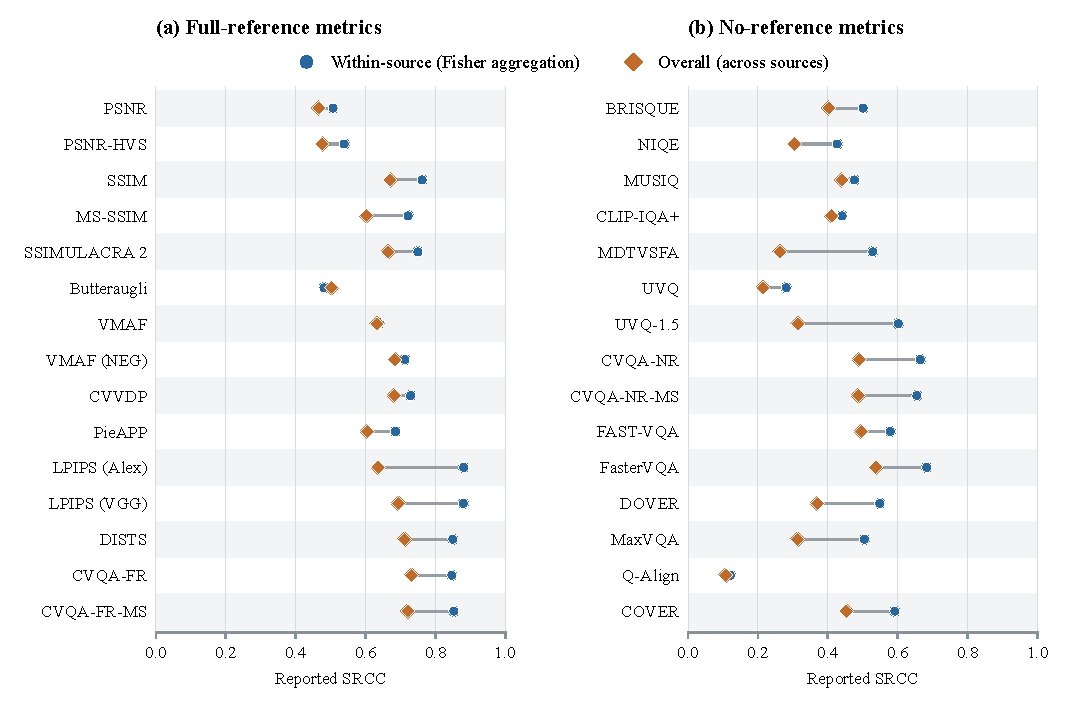
\includegraphics[width=\textwidth]{figures/benchmark.pdf}
\caption{Reported agreement between objective predictions and subjective scores for diffusion-based VSR. All 30 SRCC pairs are redrawn from Herb et al.~\cite{metric}, Table I, in the original table order. Circles show within-source correlations aggregated by Fisher transformation; diamonds show overall correlations across sources. Lines connect the two reported values for a metric, rather than uncertainty intervals. The study retains 28 observers and uses six source clips; the reported values and sign conventions are preserved. Table I supplies no SRCC confidence intervals. These results characterize the study's tested content and configurations.}
\label{fig:metriccorrelations}
\end{figure*}

Neural full-reference predictors provide useful ranking information in this experiment, while no-reference predictors can overrate some oversharpened outputs and pixel metrics are sensitive to small spatial misalignments. These findings support combining objective scores with subjective assessment, particularly when generative detail changes the appearance of a scene. The observed ranking remains specific to the tested content, degradations, methods, and viewing conditions; it does not establish a universal ordering of quality metrics across restoration domains.

Model configuration also influences the interpretation of the study. To fit an A100 with 40 GB memory, the authors adjust temporal batches, overlap, and spatial processing where necessary. These choices can affect temporal consistency and runtime as well as feasibility. The reported timings therefore characterize the evaluated configurations and cannot be transferred directly to methods running with different processing windows or hardware. This illustrates the close relationship between visual quality, implementation choices, and resource constraints in diffusion-based VSR.

\subsection{Fair Comparison Across Backbones}
Restoration methods increasingly draw on different pretrained image and video models, whose training data, capacity, temporal representations, and generative quality vary substantially. Comparing their final outputs reveals useful system-level progress, but does not by itself isolate the contribution of a restoration mechanism. A shared model family also does not guarantee matched pretraining or initialization. These differences motivate separating controlled comparison from comparison of complete systems.

\textbf{Controlled comparison.} This track examines conditioning strategies, temporal coupling, objectives, or samplers under matched resources. A common prior checkpoint, training-data access, degradation protocol, resolution, temporal context, sampling budget, and side information reduce confounding factors. Total and trainable parameter counts account for auxiliary components such as adapters, decoders, and flow networks. Some mechanisms are closely tied to a particular backbone and cannot be transferred without changing their operation. In those cases, matched ablations within the original system provide more interpretable evidence than a nominally shared backbone that alters the method itself.

\textbf{Complete-system comparison.} This track retains each system's intended backbone and training recipe while using common test clips and evaluation conditions. It measures the quality--cost operating points available in practice. Model capacity, training data, external references, temporal context, and the computational cost of auxiliary components remain relevant explanatory variables. Such comparisons reveal the benefits of integrating stronger priors and restoration designs, although the resulting differences cannot be attributed exclusively to one architectural or algorithmic component.

The tracks address complementary questions. Controlled comparison supports analysis of restoration mechanisms; complete-system comparison captures advances in available models and their practical deployment. Together, they avoid interpreting all gains from stronger pretraining as gains from a new mechanism, while allowing the survey of system progress to include current backbones.

\subsection{Evaluation Practice}
Reproducibility in diffusion-based video restoration depends on both the model and the inference procedure. Checkpoint versions, training-data access, auxiliary models, and available conditioning determine the information used for restoration. Sampling steps, guidance, stochastic seeds, temporal windows, spatial tiles, and overlap determine how that information is processed. For long or streaming videos, future-frame access, cache behavior, and state resets further affect latency and temporal continuity. Reporting these settings alongside metric preprocessing, hardware, precision, and timing boundaries makes comparisons interpretable across implementations.

Human assessment separates questions that an overall preference may combine: viewing quality, preservation of source content, and temporal artifacts. Whether observers see the degraded input, a clean reference, both, or neither changes the judgment being elicited. Anonymized methods, randomized presentation, and documented playback and display conditions reduce avoidable variation. Subjective assessment is especially valuable for real degraded or generated videos, where a reliable reference may be unavailable, and for generative artifacts that existing quality models represent poorly.

Statistical analysis likewise reflects the structure of video data. Neighboring frames are correlated, making sequence- or content-level resampling more informative than treating every frame as an independent observation. Observer variation contributes additional uncertainty in subjective experiments. Aggregate results gain interpretability from analyses of large motion, occlusion, fine text, scene cuts, and severe degradation. For stochastic restorers, common seed sets and variation across repeated outputs distinguish reliable improvements from favorable individual samples.

Finally, quality models require validation beyond the restoration systems and content used for their calibration. Held-out model families and degradation processes test whether a predictor remains useful when the characteristic artifacts change. At the method level, reporting fidelity, perceptual quality, temporal stability, and cost separately exposes operating points and trade-offs that a single weighted score may conceal. This multidimensional view connects evaluation directly to the central objectives of diffusion-based video restoration.

\section{Challenges and Future Directions}
\label{sec:outlook}
\subsection{Balancing Fidelity, Perceptual Quality, and Temporal Consistency}
Generative priors are most useful when observations are severely degraded, yet this is also where the reconstructed detail is most ambiguous. Strong conditioning can preserve scene structure while limiting texture synthesis; a more expressive sampling process can improve appearance but introduce spatial or temporal variation. The remaining challenge is to control which information comes from the observation and which is supplied by the prior, without reducing all three quality objectives to one fixed loss weight.

An effective approach should allocate uncertainty over coherent objects and trajectories. For example, several plausible reconstructions of an occluded surface can be acceptable, whereas its texture should remain consistent when it reappears within one reconstructed video. Trajectory-aware uncertainty, confidence-conditioned guidance, and explicit identity or structural constraints offer promising directions. Controllable restoration strength could further support different applications, allowing users to adjust perceptual detail while preserving selected attributes such as motion, text, or low-frequency structure.

\subsection{Reliable Temporal Modeling for Long Videos}
Image priors require mechanisms to connect independently modeled frames, while video priors bring motion knowledge learned from large datasets~\cite{svd,wan}. Both approaches face a distinction between plausible motion and the actual motion in the input. Correspondence becomes unreliable under heavy blur, darkness, occlusion, and atmospheric distortion, and attention can associate visually similar but unrelated regions. Combining correspondence uncertainty with learned temporal representations may improve robustness under these conditions.

Long videos create additional challenges. A model must maintain identity across temporary occlusion, recover context after viewpoint changes, and reset state at scene boundaries. Recurrent memory and attention caches reduce computation but can propagate early reconstruction errors. Future work should investigate selective state updates, motion-aware memory, and re-anchoring to current observations. Evaluation on long trajectories and scene transitions will be necessary to connect improvements in short-clip consistency to sustained performance.

\subsection{Unified and Fair Evaluation}
The diversity of backbones, pretraining data, degradation models, and inference settings makes it difficult to attribute improvements to a particular restoration technique. Controlled comparisons using shared initialization and matched data can reveal the value of conditioning or temporal modules, while complete-system comparisons capture practical advances from larger priors and optimized implementations. A common benchmark should support both forms of comparison and cover synthetic, real, specialized, and generated-video inputs.

Metric reliability remains equally important. Subjective assessment of diffusion-based VSR reveals different behavior across reference-based and no-reference predictors, and between within-source and overall evaluation~\cite{metric}. As generators produce sharper and smoother outputs, their remaining errors may involve identity, geometry, and motion rather than conventional blur or noise. New quality models should separate perceptual preference from source fidelity and temporal correctness, with evaluation across unseen restorers and degradations. Human judgments remain valuable for understanding these dimensions and calibrating objective measures.

\subsection{Broader Tasks and Physically Grounded Restoration}
Natural-video super-resolution has provided a productive setting for developing diffusion restoration. Weather removal, underwater enhancement, infrared restoration, face restoration, and event-guided processing demonstrate the broader potential of generative priors~\cite{difftta,weatherweaver,undive,hatir,flair,evdiffuser}. Extending these methods to diverse acquisition conditions requires a closer relationship between model design and image formation. Unknown mixtures such as scattering with motion blur, changing underwater illumination, or low-light compression can violate the assumptions of models trained on simpler degradations.

Physical modeling and multimodal observations provide complementary information. Events can constrain fast motion, reference images can preserve identity, and sensor metadata can inform noise or exposure models. Their integration should account for calibration errors, missing modalities, and changing conditions. HDR and infrared restoration also require objectives that preserve radiometric or thermal structure rather than merely reproducing the appearance of natural RGB video. Progress in these domains will depend on suitable data, models, and task-specific evaluation.

\subsection{Efficient Inference Beyond Sampling Steps}
One-step and few-step methods reduce the cost of repeated denoising, but high-resolution video processing can remain dominated by autoencoders, attention, tiling, and temporal overlap~\cite{dove,seedvr2,flash}. Efficiency therefore requires joint optimization of the full restoration system. Restoration-aware compression, lightweight temporal decoders, sparse attention, and reusable state offer opportunities to reduce cost while retaining detail and temporal coherence.

Streaming introduces a further balance between context and delay. Future frames improve reconstruction in offline processing, whereas online applications must operate with limited look-ahead. Adaptive computation could allocate more resources to difficult motion, occlusion, or degradation transitions while processing easier segments cheaply. Such strategies should be evaluated using first-output latency, sustained throughput, peak memory, and long-horizon quality, rather than denoising step count alone.

\subsection{Generalist and Adaptive Restoration Systems}
A single restoration model must accommodate degradations with different physical causes and potentially conflicting objectives. Prompts, expert routing, and shared representations provide ways to combine specialization with parameter sharing, but generalization to unfamiliar mixtures remains challenging. Continual adaptation and self-supervised learning may help models respond to changing cameras and environments without requiring paired clean video for every condition.

Agentic restoration extends adaptation to the choice and ordering of operators. Its effectiveness depends on diagnosing degradation, selecting compatible models, and deciding when further enhancement would damage content. Quality feedback can support this process, but an evaluator that rewards oversharpening or invented detail can also reinforce errors. Future systems should combine perceptual feedback with source-consistency constraints, maintain temporal decisions across a sequence, and avoid unnecessary repeated processing. For identity-sensitive and scientific applications, the ability to preserve trustworthy content is as important as the ability to generate convincing detail.

\section{Conclusion}
Diffusion models have expanded video restoration and enhancement through powerful image and video priors, flexible conditioning, and increasingly efficient inference. This survey has organized their development by prior source, learning strategy, temporal mechanism, task, and system paradigm. Across these categories, the central challenge is to connect synthesized detail to the observed scene while preserving coherent appearance and motion over time.

Further progress will require joint advances in restoration control, long-video modeling, domain-specific learning, and evaluation. Shared benchmarks can clarify the contribution of new methods, while calibrated metrics and human assessment can distinguish perceptual improvement from faithful reconstruction. Addressing these issues will support diffusion-based restoration systems that are both visually effective and reliable across diverse video applications.

\bibliographystyle{IEEEtran}
\bibliography{refs}
\end{document}
